% arara: xelatex
% arara: biber
% arara: xelatex: { synctex: true }

\documentclass[12pt,a4paper,oneside,final]{report}

\setlength\paperheight{297mm}
\setlength\paperwidth{210mm}


\usepackage{polyglossia}
\setmainlanguage[numerals=cyrillic]{russian}
\setotherlanguages{english}

\usepackage{xunicode} % some extra unicode support
%\usepackage[utf8x]{inputenc}
\usepackage{xltxtra} % \XeLaTeX macro
\usepackage{fontspec}
\defaultfontfeatures{Ligatures=TeX}

%\setromanfont{Charis SIL}
%\setsansfont{Liberation Sans}
%\setmonofont{PT Mono}
%\setmainfont{Liberation Serif} % this allows to use sans-serif as default font

\usepackage{ifplatform}

\ifwindows
  \newfontfamily{\cyrillicfont}{Times New Roman}
  \setmainfont{Times New Roman}
  \newfontfamily{\cyrillicfonttt}{Courier New}
  \setmonofont{Courier New}
\else
  \setmainfont{Linux Libertine O}
  \setsansfont{Linux Biolinum O}
  \setmonofont[SmallCapsFont={Latin Modern Mono Caps}]{Latin Modern Mono Light}
\fi

%нумерация справа и колонтитулы справа вверху
\usepackage{fancyhdr}
\usepackage[left=25mm,right=10mm,top=20mm,bottom=20mm,bindingoffset=0cm]{geometry}%

\usepackage{amsfonts}
\usepackage{amssymb}
\usepackage{amsmath}
\usepackage{amsthm}

\usepackage{calc}
\usepackage{ifthen}
\usepackage{graphicx}
\usepackage{array}
\usepackage{pdfpages}
\usepackage{longtable}
\usepackage{tabu}
\usepackage{indentfirst}
\usepackage[unicode=true]{hyperref}
\usepackage{color}
\usepackage{pgf}

\usepackage{pstheorems}

% Настройка списков (без лишних вертикальных отступов)
\usepackage{paralist}
\setdefaultenum{1.}{1.}{1.}{1.}
\setdefaultitem{--}{}{}{}
%\setlength\itemsep{-1em}
\let\itemize\compactitem
\let\enditemize\endcompactitem
\let\enumerate\compactenum
\let\endenumerate\endcompactenum
\let\description\compactdesc
\let\enddescription\endcompactdesc
\pltopsep=\smallskipamount
\plitemsep=0pt
\plparsep=0pt
% Команда для отмены разрыва страниц перед списками
\makeatletter 
\newcommand\mynobreakpar{\par\nobreak\@afterheading} 
\makeatother
%%%%%%

\usepackage[singlelinecheck=false,labelsep=endash]{caption}
\captionsetup[table]{justification=justified}
\captionsetup[figure]{justification=centering}

\usepackage{titlesec}
\titleformat{\chapter}[block]{\centering\normalfont\Large\bfseries}{\thechapter.}{1ex}{}{}
\titlespacing{\chapter}{0pt}{0em}{2em}

\titleformat{\section}[block]{\normalfont\large\bfseries}{\thesection}{1ex}{}{}
\titlespacing{\section}{0pt}{0em}{1ex}

\titleformat{\subsection}[block]{\normalfont\normalsize\bfseries}{\thesubsection}{1ex}{}{}
\titlespacing{\section}{0pt}{0em}{1ex}

	% paragraph и subparagraph -- в тексте, без отступов
\titleformat{\paragraph}[runin]{\normalfont\normalsize\bfseries}{\theparagraph}{0pt}{}{}
\titlespacing{\paragraph}{0pt}{0em}{0ex}

\titleformat{\subparagraph}[runin]{\normalfont\normalsize\bfseries}{\thesubparagraph}{0pt}{}{}
\titlespacing{\subparagraph}{0pt}{0em}{0ex}


% Своё название для Cписка литературы
\usepackage[title, titletoc]{appendix}
\addto\captionsrussian{% Replace "english" with the language you use
	\renewcommand{\contentsname}%
	{Содержание}%
}

%\renewcommand{\appendixname}{Приложение}% Change "chapter name" for Appendix chapters
%\renewcommand{\cftchapdotsep}{\cftdotsep}

\usepackage{mathpartir}

\makeatletter
\let\ps@plain\ps@fancy              % Подчиняем первые страницы каждой главы общим правилам
\makeatother
\pagestyle{fancy}
\fancyhf{}
\fancyfoot[C]{\thepage}
\renewcommand{\headrulewidth}{0pt}
\renewcommand{\footrulewidth}{0pt}
\renewcommand{\baselinestretch}{1.5}
\newcommand{\headertext}[1]{\fancyhead[R]{\tiny{#1}}}

%% Список литературы

\makeatletter
\bibliographystyle{ugost2008}     % Оформляем список литературы по ГОСТ 7.1
% (ГОСТ Р 7.0.11-2011, 5.6.7)
\renewcommand{\@biblabel}[1]{#1.}   % Заменяем список литературы с квадратных
% скобок на точку
\makeatother

%\frenchspacing %% изменение расстояние до и после точек в ряде случаев

\renewcommand{\theenumi}{\arabic{enumi}}
\renewcommand{\theenumii}{\arabic{enumii}}
\renewcommand{\theenumiii}{\arabic{enumiii}}
\renewcommand{\theenumiv}{\arabic{enumiv}}

\renewcommand{\labelenumi}{\theenumi.}
\renewcommand{\labelenumii}{\theenumi.\theenumii.}
\renewcommand{\labelenumiii}{\theenumi.\theenumii.\theenumiii.}
\renewcommand{\labelenumiv}{\theenumi.\theenumii.\theenumiii.\theenumiv.}

%\newenvironment{annotation}{\textbf{Аннотация.} \textit}{}
\theoremstyle{plain}
\newtheorem*{annotation}{Аннотация}

\usepackage{listingsutf8}

\renewcommand{\lstlistingname}{Листинг}

\lstset{
  basicstyle=\linespread{0.94}\ttfamily\small,
  tabsize=2,
  showstringspaces=false,
  columns=flexible,
  numbers=none,
  numberstyle=\tiny\color{gray},
  breaklines=true,
  breakatwhitespace=true,
  framesep=6pt,
  abovecaptionskip=1em,
  captionpos=b,
  extendedchars=true,
  inputencoding=utf8,
  literate={Ö}{{\"O}}1
  {Ä}{{\"A}}1
  {Ü}{{\"U}}1
  {ß}{{\ss}}1
  {ü}{{\"u}}1
  {ä}{{\"a}}1
  {ö}{{\"o}}1
  {~}{{\textasciitilde}}1
  {а}{{\selectfont\char224}}1
  {б}{{\selectfont\char225}}1
  {в}{{\selectfont\char226}}1
  {г}{{\selectfont\char227}}1
  {д}{{\selectfont\char228}}1
  {е}{{\selectfont\char229}}1
  {ё}{{\"e}}1
  {ж}{{\selectfont\char230}}1
  {з}{{\selectfont\char231}}1
  {и}{{\selectfont\char232}}1
  {й}{{\selectfont\char233}}1
  {к}{{\selectfont\char234}}1
  {л}{{\selectfont\char235}}1
  {м}{{\selectfont\char236}}1
  {н}{{\selectfont\char237}}1
  {о}{{\selectfont\char238}}1
  {п}{{\selectfont\char239}}1
  {р}{{\selectfont\char240}}1
  {с}{{\selectfont\char241}}1
  {т}{{\selectfont\char242}}1
  {у}{{\selectfont\char243}}1
  {ф}{{\selectfont\char244}}1
  {х}{{\selectfont\char245}}1
  {ц}{{\selectfont\char246}}1
  {ч}{{\selectfont\char247}}1
  {ш}{{\selectfont\char248}}1
  {щ}{{\selectfont\char249}}1
  {ъ}{{\selectfont\char250}}1
  {ы}{{\selectfont\char251}}1
  {ь}{{\selectfont\char252}}1
  {э}{{\selectfont\char253}}1
  {ю}{{\selectfont\char254}}1
  {я}{{\selectfont\char255}}1
  {А}{{\selectfont\char192}}1
  {Б}{{\selectfont\char193}}1
  {В}{{\selectfont\char194}}1
  {Г}{{\selectfont\char195}}1
  {Д}{{\selectfont\char196}}1
  {Е}{{\selectfont\char197}}1
  {Ё}{{\"E}}1
  {Ж}{{\selectfont\char198}}1
  {З}{{\selectfont\char199}}1
  {И}{{\selectfont\char200}}1
  {Й}{{\selectfont\char201}}1
  {К}{{\selectfont\char202}}1
  {Л}{{\selectfont\char203}}1
  {М}{{\selectfont\char204}}1
  {Н}{{\selectfont\char205}}1
  {О}{{\selectfont\char206}}1
  {П}{{\selectfont\char207}}1
  {Р}{{\selectfont\char208}}1
  {С}{{\selectfont\char209}}1
  {Т}{{\selectfont\char210}}1
  {У}{{\selectfont\char211}}1
  {Ф}{{\selectfont\char212}}1
  {Х}{{\selectfont\char213}}1
  {Ц}{{\selectfont\char214}}1
  {Ч}{{\selectfont\char215}}1
  {Ш}{{\selectfont\char216}}1
  {Щ}{{\selectfont\char217}}1
  {Ъ}{{\selectfont\char218}}1
  {Ы}{{\selectfont\char219}}1
  {Ь}{{\selectfont\char220}}1
  {Э}{{\selectfont\char221}}1
  {Ю}{{\selectfont\char222}}1
  {Я}{{\selectfont\char223}}1
  {…}{\ldots}1
  {–}{-}1
  {\ }{ }1
}

\authorgroup{Б20-524}
\author{Корначук М. В.}
\authorfulldative{Корначуку Марку Всеволодовичу}
\supervisor{Шапкин П. А.}
\consultant{$\emptyfield$}
\projecttypefulldative{учебно-исследовательской работе}
\projecttypeshort{УИР}

\title{Исследование и реализация сферического коня в вакууме\\
  на основе теоретико-множественного подхода}

\taskdate{01.09.2020}

\projecttasks{
  \projecttask{\bfseries\projecttasknum}{\bfseries Аналитическая часть}{}{}{}
    % (указываются предмет и цели анализа)
    \projecttask{\projectsubtasknum}
      {Изучение и сравнительный анализ … с целью…}%
      {Аналитический отчет, список литературы}%
      {}{\signat[4pt]{.12}{VGPetrov}{01.01.2001}}
    \projecttask{\projectsubtasknum}
      {Изучение и анализ … для…}%
      {}%
      {}{}
    \projecttask{\projectsubtasknum}
      {Анализ … применительно к задачам…}%
      {}%
      {}{}
    \projecttask{\projectsubtasknum}
      {Анализ возможностей… (для…, применительно к…, и т.п.)}%
      {}%
      {}{}
    \projecttask{\projectsubtasknum}
      {Оформление расширенного содержания пояснительной записки (РСПЗ)}%
      {Текст РСПЗ}%
      {20.10.2020}{}
  \projecttask{\bfseries\projecttasknum}{\bfseries Теоретическая часть}{}{}{}
    % (указываются используемые и разрабатываемые модели, методы, алгоритмы)
    \projecttask{\projectsubtasknum}
      {Используется … (модель, метод, алгоритм(ы)…) Модель/ алгоритм/метод...}%
      {}%
      {}{}
    \projecttask{\projectsubtasknum}
      {Выбор/разработка…}%
      {}%
      {}{}
    \projecttask{\projectsubtasknum}
      {Разработка…}%
      {}%
      {}{}
    \projecttask{\projectsubtasknum}
      {Модификация… (алгоритма, модели, и т.п.) для …}%
      {}%
      {}{}
    \projecttask{\projectsubtasknum}
      {Адаптация … для…}%
      {}%
      {}{}
  \projecttask{\bfseries\projecttasknum}{\bfseries Инженерная часть}{}{}{}
    % (указывается, что конкретно необходимо спроектировать, а также используемые для этого методы, технологии и инструментальные средства)
    \projecttask{\projectsubtasknum}
      {Проектирование … (системы, подсистемы, модуля…)}%
      {}%
      {}{}
    \projecttask{\projectsubtasknum}
      {Использовать методологию проектирования….}%
      {}%
      {}{}
    \projecttask{\projectsubtasknum}
      {Разработать архитектуру для… (с учетом требований к…)}%
      {}%
      {}{}
    \projecttask{\projectsubtasknum}
      {Результаты проектирования оформить с помощью…. При проектировании использовать язык… (например, IDEF, или UML)}%
      {}%
      {}{}
  \projecttask{\bfseries\projecttasknum}{\bfseries Технологическая и практическая часть}{}{}{}
    % (указывается, что конкретно должно быть реализовано и протестировано, а также используемые для этого методы, инструментальные средства, технологии)
    \projecttask{\projectsubtasknum}
      {Реализовать… (систему, подсистему, модуль…)}%
      {Исполняемые файлы, исходный текст}%
      {}{}
    \projecttask{\projectsubtasknum}
      {Протестировать… с помощью…}%
      {}%
      {}{}
    \projecttask{\projectsubtasknum}
      {Разработать тестовые примеры для… }%
      {Исполняемые файлы, исходные тексты тестов и тестовых примеров}%
      {}{}
    \projecttask{\projectsubtasknum}
      {Реализация должна иметь форму/обладать качествами...}%
      {}%
      {}{}
    \projecttask{\projectsubtasknum}
      {Ожидаемым результатом является программная система/программный комплекс/программное обеспечение… со следующими отличительными характеристиками…}%
      {}%
      {}{}
    \projecttask{\projectsubtasknum}
      {При реализации использовать технологию/платформу…}%
      {}%
      {}{}
  \projecttask{\bfseries\projecttasknum}
    {\bfseries Оформление пояснительной записки (ПЗ) и иллюстративного материала для доклада.}%
    {\bfseries Текст ПЗ, презентация}%
    {\bfseries 15.12.2021}{}
}

\taskliterature{
\nocite{Sychev}
\nocite{Sokolov}
\nocite{Gaidaenko}
}

% # Подписи

% Для простановки подписи используются слдеющие команды:
% - простая подпись: \sign[<сдвиг>]{<масштаб>}{<FIO>}
% - подпись с датой: \signat[<сдвиг>]{<масштаб>}{<FIO>}{<дата>}
% где
% - <сдвиг> --- необязательный сдвиг подписи по вертикали для правильного
%   расположения относительно строки
% - <масштаб> --- число, используемое для масштарибования изображения подписи
% - <FIO> --- имя файла с подписью, файл должен быть помещен в
%   img/signatures/FIO.png и иметь прозрачный фон
% - <дата> --- дата, которая будет выведена под подписью

% ## Утверждение задания руководителем и студентом
\authortaskapproval{\sign[10pt]{.15}{ABIvanov}}
\supervisortaskapproval{\sign[10pt]{.15}{VGPetrov}}

% ## Утверждение РСПЗ руководителем, студентом и консультантом
\authorrspzapproval{\sign[10pt]{.15}{ABIvanov}}
\supervisorrspzapproval{\sign[10pt]{.15}{VGPetrov}}
\consultantrspzapproval{}

% ## Оценка руководителя за РСПЗ
\supervisorrspzgrade{10}

% ## Утверждение ПЗ руководителем, студентом и консультантом
\authorpzapproval{}
\supervisorpzapproval{\sign[10pt]{.15}{VGPetrov}}
\consultantpzapproval{}

% ## Оценка руководителя за ПЗ
\supervisorpzgrade{12}


\headertext{}

\addto{\captionsrussian}{\renewcommand{\bibname}{Список литературы}}

\begin{document}

\documenttype{Расширенное содержание пояснительной записки}
% \documenttype{Пояснительная записка}

% Для титульного листа, сверстанного в LaTeX
\pagestyle{empty}
\begin{center}
  {\scriptsize
    \uppercase{Министерство науки и высшего образования российской федерации}\linebreak
    \uppercase{Федеральное государственное автономное образовательное
    учреждение высшего образования}
  }

  \textbf{Национальный исследовательский ядерный университет «МИФИ»}

  {\footnotesize
    \noindent\makebox[\linewidth]{\rule{\linewidth}{0.4pt}}
  }
\end{center}

\vskip 1em

\sloppy

\noindent
\begin{tabular}{@{}lc@{}}
\multirow{2}{*}{
\includegraphics[width=0.2\linewidth]{mephi.png}}
  & \textbf{\large{}Институт интеллектуальных кибернетических систем} \\
  & \uppercase{\textbf{\large{}Кафедра кибернетики (№ 22)}}  \\
\end{tabular}
\fussy


\vfill

\begin{center}
  Направление подготовки 09.03.04 Программная инженерия

  \vfill

  {\Large{\textbf{\thedocumenttype}}}

  к учебно-исследовательской работе студента на тему:

  {\Large\thetitle}
\end{center}

\vfill

{\large

\noindent
\begin{tabular}{@{}lll@{}}
Группа              & \theauthorgroup      &  \\   
Студент             & $\rule{5cm}{0.15mm}$ & \theauthor \\    
Руководитель        & $\rule{5cm}{0.15mm}$ & \thesupervisor \\         
Научный консультант & $\rule{5cm}{0.15mm}$ & \theconsultant \\                
\end{tabular}

\vfill

\noindent
Оценка руководителя \quad $\rule{3cm}{0.15mm}$ \quad
Оценка комиссии     \quad $\rule{3cm}{0.15mm}$

\vfill

\noindent
\begin{tabular}{@{}lcc@{}}
Члены комиссии & & \\
& $\rule{6cm}{0.15mm}$ & $\rule{6cm}{0.15mm}$ \\
& $\rule{6cm}{0.15mm}$ & $\rule{6cm}{0.15mm}$ \\
& $\rule{6cm}{0.15mm}$ & $\rule{6cm}{0.15mm}$ \\
& $\rule{6cm}{0.15mm}$ & $\rule{6cm}{0.15mm}$ \\
\end{tabular}

\vfill

\begin{center}
\textbf{Москва \the\year}
\end{center}

}

\newpage

% Для вставки бланка титульного листа из PDF-файла
% 
\includepdf[pages={-}, offset=0mm -0mm]{title/title.pdf}

%\clearpage
%% Тут включается лист с подписями для ВКР
%
\includepdf[pages={-}, offset=0mm -0mm]{title/title-dep22.pdf}
%\clearpage

% Для листа задания, сверстанного в LaTeX
\pagestyle{empty}
\begin{center}
  {\scriptsize
    \uppercase{Министерство науки и высшего образования российской федерации}\linebreak
    \uppercase{Федеральное государственное автономное образовательное
    учреждение высшего образования}
  }

  \textbf{Национальный исследовательский ядерный университет «МИФИ»}

  {\footnotesize
    \noindent\makebox[\linewidth]{\rule{\linewidth}{0.4pt}}
  }
\end{center}

\vskip 1em

\sloppy

\noindent
\begin{tabular}{@{}lc@{}}
\multirow{2}{*}{
\includegraphics[width=0.2\linewidth]{mephi.png}}
  & \textbf{\large{}Институт интеллектуальных кибернетических систем} \\
  & \uppercase{\textbf{\large{}Кафедра кибернетики (№ 22)}}  \\
\end{tabular}
\fussy


\begin{center}
  {\Large{\textbf{Задание на \theprojecttypeshort}}}\\

  \large

  Студенту гр. \theauthorgroup{} \theauthorfulldative
\end{center}

\begin{center}
  \uppercase{\textbf{\large{}Тема \theprojecttypeshort}}\\

  {\Large\thetitle}\\

  \vskip 1em

  \uppercase{\textbf{\large{}Задание}}
\end{center}

{\linespread{1.0}
  \footnotesize
  \noindent
  \begin{longtable}{|p{.5cm}|p{230pt}|>{\scriptsize\centering\arraybackslash}p{2cm}|>{\centering\arraybackslash}p{2cm}|>{\centering\arraybackslash}p{2cm}|} \hline
  \multicolumn{1}{|>{\centering\arraybackslash}p{0.5cm}|}{№\par п/п}
    & \multicolumn{1}{c|}{Содержание работы}
    & {\footnotesize Форма отчетности}
    & Срок исполнения
    & Отметка о выполнении\par {\scriptsize Дата, подпись} \\\hline
  \theprojecttasks
  \end{longtable}
}
\refsection
\thetaskliterature
\begin{center}
  \uppercase{\textbf{\large{}Литература}}
\end{center}
\printbibliography[heading=none]
\endrefsection

\vfill

{\noindent\linespread{2.0}
  \begin{tabularx}{\linewidth}{p{140pt}X>{\centering}XX}
    Дата выдачи задания: & Руководитель & \thesupervisortaskapproval & \thesupervisor \\ \hhline{~~-~}
    \thetaskdate         & Студент      & \theauthortaskapproval     & \theauthor     \\ \hhline{~~-~}
  \end{tabularx}
}

\newpage

% Для вставки бланка задания из PDF-файла
% 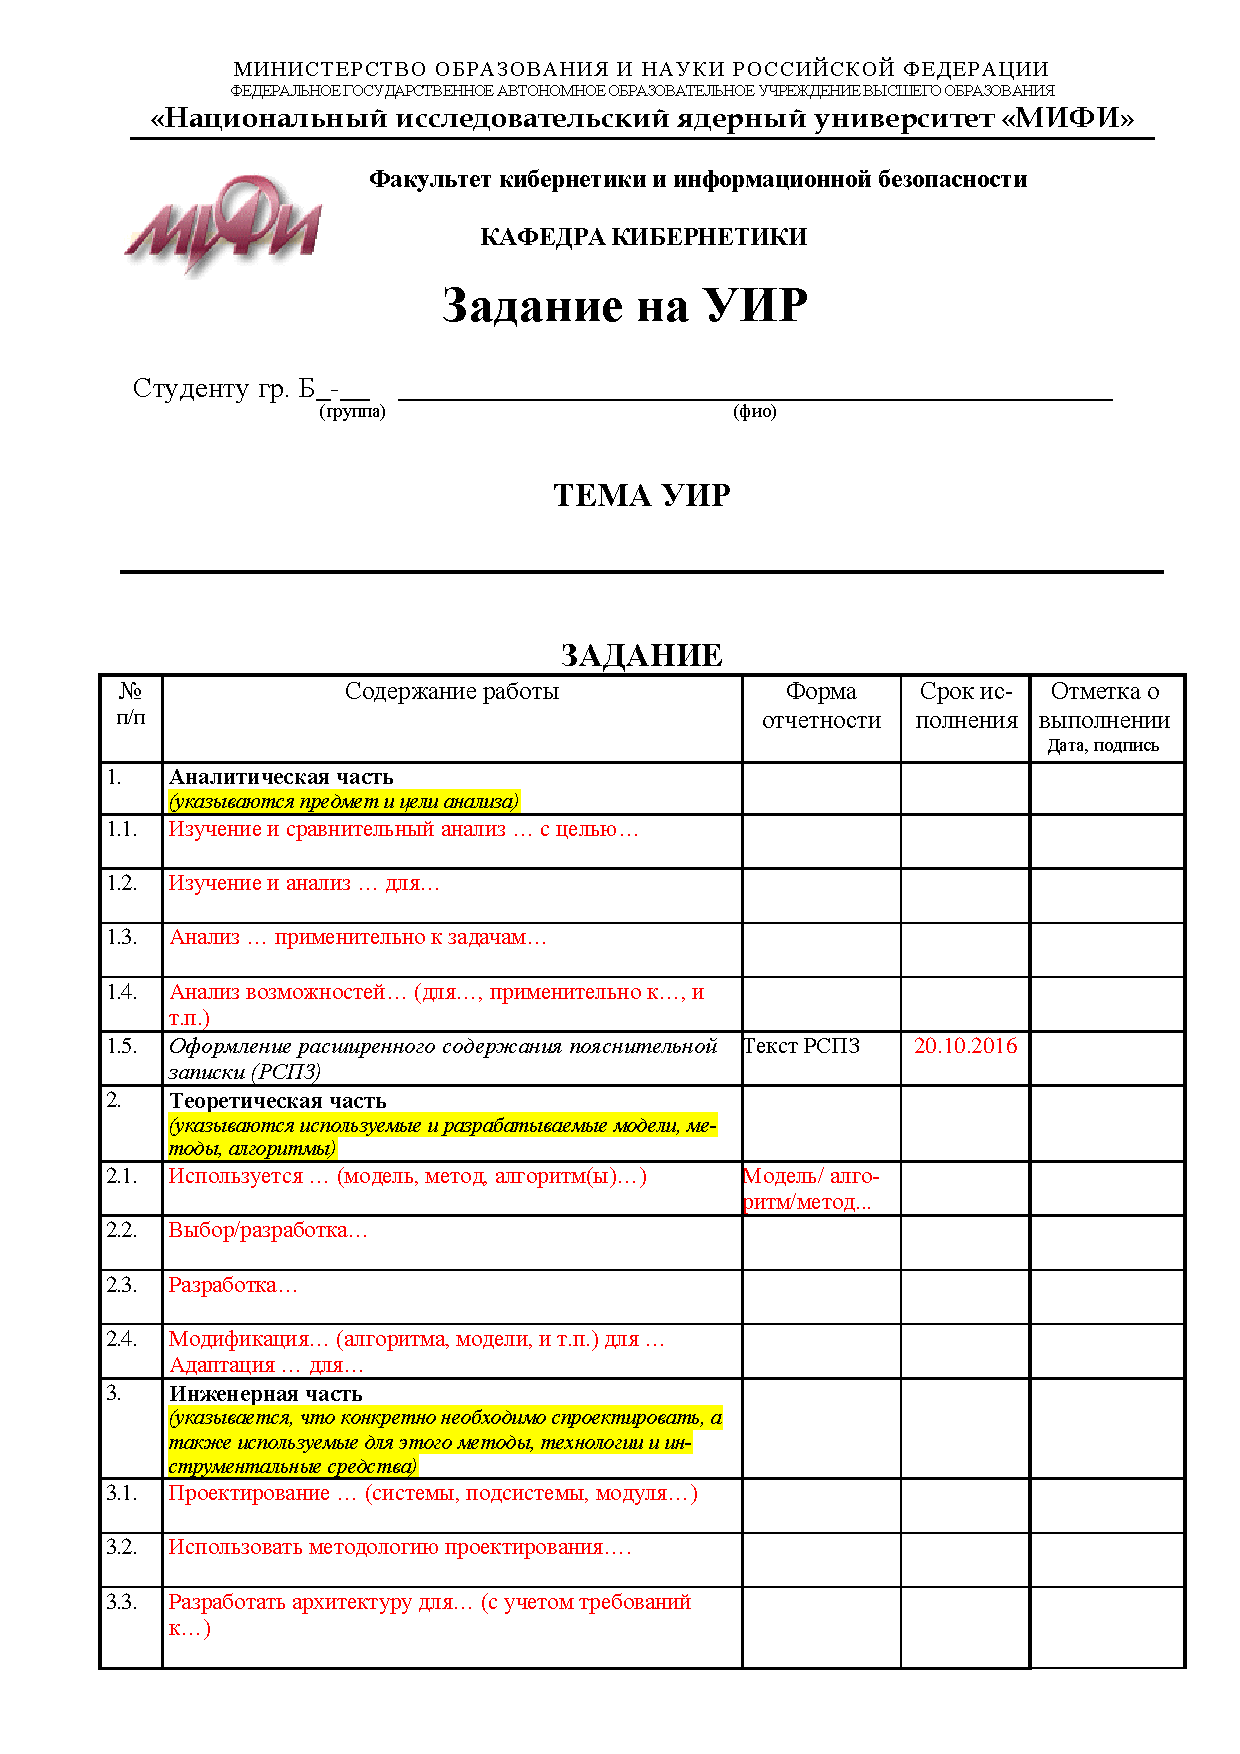
\includepdf[pages={-}, offset=0mm -0mm]{title/task.pdf}

\pagenumbering{arabic}

\refsection

%\clearpage
%\thispagestyle{empty}

%\vfill

%\begin{center}
%[Место для распечатки отчета Антиплагиата]
%\end{center}

%\newpage
%\thispagestyle{empty}

%\vfill

%\begin{center}
%[Место для распечатки отчета Антиплагиата]
%\end{center}

\clearpage

\chapter*{Реферат}
\thispagestyle{plain}

Общий объем основного текста, без учета приложений ---
\pageref{end_of_main_text} страниц, с учетом приложений ---
\pageref{end_of_document}. Количество использованных источников~--- ХХ.
Количество приложений~--- Х.

Ключевые слова: \dots .

Целью данной работы является \dots

В первой главе проводится обзор и анализ \dots 

Во второй главе описываются использованные и разработанные/модифицированные методы/модели/алгоритмы \dots. 

В третьей главе приводится описание программной реализации и экспериментальной проверки \dots.

В приложении \ref{app-format} описаны основные требования к форматированию пояснительных записок к дипломам и (магистерским) диссертациям.

В приложении \ref{app-structure} представлена общая структура пояснительной записки.

В приложении \ref{app-manual} приведены некоторые дополнительные комментарии к использованию данного шаблона.


\clearpage

\tableofcontents{}

\clearpage

\chapter*{Введение}
\label{sec:afterwords}
\addcontentsline{toc}{chapter}{Введение}

Эффективное управление и автомасштабирование кластеров Kubernetes в облачных
средах играют ключевую роль в современной информационной инфраструктуре.
Актуальность этой темы подчеркивается быстрым развитием технологий в области
облачных вычислений и необходимостью адаптации к постоянно меняющимся
требованиям рынка. В данном контексте, особое внимание уделяется системам, таким
как Terraform и Scala, для обеспечения надежного и гибкого управления
инфраструктурой.

Цель данной работы - доработка и тестирование системы автомасштабирования
кластера Kubernetes на платформе Яндекс Облако. Основной акцент сделан на
интеграции Terraform, инструмента для управления инфраструктурой как кодом, и
Scala, языка программирования, который предоставляет мощные возможности для
типизации и модульного программирования. Эта работа направлена на оптимизацию и
усовершенствование существующих типизированных структур, которые обеспечат
гибкость, эффективность и стабильность в процессах автоматизации и управления.

Новизна данной работы заключается в доработке и оптимизации системы
автомасштабирования кластера Kubernetes, сочетающей функциональные возможности
Terraform и Scala для обеспечения улучшенной производительности,
масштабируемости и стабильности в облачных средах.

Оригинальность исследования проявляется в разработке усовершенствованного
подхода к автомасштабированию, сочетающего эффективность Terraform в
автоматизации развертывания инфраструктуры с расширенными функциональными
возможностями и статической типизацией языка Scala.

Целью работы является доработка и тестирование системы автомасштабирования
кластера Kubernetes, с акцентом на следующие задачи:

\begin{enumerate}
\item Проанализировать результаты предыдущего этапа работы и определить
направления для доработки и оптимизации системы автомасштабирования.
\item Разработать улучшенный алгоритм автомасштабирования с учетом новых
возможностей и обновлений в используемых технологиях.
\item Оптимизировать модель данных для более эффективного мониторинга и
управления ресурсами Kubernetes.
\item Провести рефакторинг кода для повышения производительности, читаемости и
поддерживаемости системы.
\item Развернуть доработанную систему автомасштабирования в тестовой среде
Kubernetes и провести тестирование для оценки эффективности улучшений.
\end{enumerate}

Первая глава посвящена анализу результатов предыдущего этапа работы и
определению направлений для доработки и оптимизации системы автомасштабирования.

Вторая глава описывает процесс разработки улучшенного алгоритма
автомасштабирования и оптимизации модели данных.

Третья глава фокусируется на доработке модуля автомасштабирования и рефакторинге
кода для повышения производительности и поддерживаемости системы.

Четвертая глава представляет результаты развертывания доработанной системы в
тестовой среде, проведения тестирования и оценки эффективности улучшений.

В заключении обобщаются результаты исследования, формулируются основные выводы и
определяются перспективы дальнейшего развития и усовершенствования системы
автомасштабирования в облачных средах.

\clearpage

\chapter{Анализ инструментов развертывания контейнеризированных
сред и возможности интеграции с Terraform и Scala}
\label{chapter1}

\section{Обоснование выбора Scala как языка реализации проекта}

Scala представляет собой мощный и гибкий язык программирования, который сочетает
в себе преимущества объектно-ориентированного и функционального
программирования. Вот несколько причин, почему Scala является хорошим выбором
для реализации проекта по развертыванию контейнеризированных приложений и
интеграции с Terraform:

1. \textbf{Статическая типизация}: Scala является статически типизированным
языком, что обеспечивает более высокую безопасность и надежность
программного кода. Статическая типизация позволяет выявить ошибки
на ранней стадии разработки и обеспечить более простое рефакторинг
и поддержку кода \cite{pierce-types-2012-ru}. Кроме того, Scala предоставляет
возможности для создания безопасных абстракций на уровне типов
\cite{moors2008safe}.

2. \textbf{Мощные возможности абстракции}: Scala предоставляет богатый
набор инструментов для создания абстракций, таких как классы,
типажи (трейты) и высокоуровневые функции. Это позволяет разработчикам
выразить сложные операции и логику в более простой и понятной форме,
повышая читаемость и поддерживаемость кода \cite{moors2008safe}.

3. \textbf{Функциональное программирование}: Scala хорошо поддерживает
функциональное программирование, что позволяет использовать
высокоуровневые абстракции, избегать изменяемого состояния и
создавать модульный и тестируемый код. Функциональный подход
особенно полезен при работе с асинхронными операциями и обработкой ошибок.

4. \textbf{Богатая экосистема}: Scala имеет широкую экосистему библиотек
и фреймворков, которые облегчают разработку и обеспечивают доступ
к множеству полезных инструментов. Например, Cats и Cats Effect
предоставляют функциональные абстракции и типажи для упрощения
работы с эффектами и асинхронным программированием
\cite{cats-effect, cats}.

5. \textbf{Интеграция с Java и JVM}: Scala полностью совместима с Java
и может взаимодействовать с существующими Java-библиотеками и
инфраструктурой. Это дает возможность использовать богатую экосистему
Java и переиспользовать существующий код и инструменты.

6. \textbf{Поддержка функционального комбинаторного программирования}:
Scala имеет поддержку для функциональной комбинаторной логики, которая
может быть полезна для моделирования и анализа систем
\cite{wolfengagen-combinatory-2008, wolfengagen-methods-2008}.
Это может быть полезно при разработке алгебраического описания для
представления объектов Terraform и других частей проекта.

В целом, Scala предлагает разработчикам мощные инструменты и гибкость,
которые могут быть полезны при реализации проекта по развертыванию
контейнеризированных приложений и интеграции с Terraform. Она позволяет
создавать высококачественный, типобезопасный и модульный код, что важно
для разработки сложных систем.

\section{Обзор системы Terraform и методов обеспечения интеграции с ней}

Terraform - это инструмент открытого исходного кода, разработанный HashiCorp,
для безопасного и эффективного управления облачной инфраструктурой как
кодом (IaC) \cite{jourdan2017infrastructure, morris2016infrastructure}.
Terraform позволяет определить и
предоставить полную инфраструктуру данных, серверов, сетей и приложений в
различных облачных сервисах, таких как AWS, Google Cloud, Azure и других, а
также в локальных средах, таких как VMware и OpenStack
\cite{howard2022terraform}.

Terraform использует декларативный подход, что означает, что вы описываете
желаемое состояние инфраструктуры, а Terraform заботится о том, как достичь
этого состояния. Это упрощает управление сложными системами и уменьшает
вероятность ошибок.

Terraform предоставляет множество провайдеров, которые позволяют
взаимодействовать с различными облачными сервисами и другими сервисами.
Каждый провайдер предоставляет набор ресурсов, которые можно управлять
с помощью Terraform. Например, провайдер AWS предоставляет ресурсы,
такие как $aws\_instance$ и $aws\_vpc$, которые можно использовать для
управления экземплярами EC2 и VPC в AWS \cite{howard2022terraform}.

Terraform поддерживает модули, что позволяет группировать и повторно
использовать ресурсы. Модули могут быть использованы для создания
абстракций высокого уровня, что упрощает управление сложными системами.

Terraform также поддерживает состояние, что позволяет отслеживать
текущее состояние инфраструктуры и применять изменения инкрементно.
Это уменьшает вероятность ошибок и упрощает управление сложными системами.

Для интеграции Terraform с другими системами, такими как Scala или
Kubernetes, можно использовать провайдеры Terraform, модули и другие
функции Terraform. Например, можно использовать провайдер Kubernetes
для управления ресурсами Kubernetes с помощью Terraform, или можно
использовать Scala для типизации всех структур
Terraform \cite{shapkin-automation-2022}, на примере того,
как это описано в данной статье, для последующей
генерации файлов конфигурации Terraform.

Важно отметить, что Terraform предоставляет множество возможностей
для автоматизации и управления облачной инфраструктурой, но он также
требует знания и понимания облачных сервисов и концепций IaC.
Поэтому важно провести тщательное исследование и планирование перед
использованием Terraform в проекте.

В заключение, Terraform представляет собой мощный инструмент для
управления облачной инфраструктурой как кодом. Он предлагает гибкость
и контроль, которые требуются для управления сложными системами,
и предоставляет множество возможностей для интеграции с другими
системами и инструментами. Однако, как и любой мощный инструмент,
он требует знания и понимания для эффективного использования.

\section{Анализ системы Kubernetes и её особенностей типизации}

Kubernetes - это открытая система для автоматизации развертывания,
масштабирования и управления контейнеризированными приложениями.
Она была разработана Google и сейчас поддерживается Cloud Native Computing
Foundation \cite{bernstein-containers-2014}.

Одной из ключевых особенностей Kubernetes является её система типов
ресурсов. В Kubernetes каждый объект, такой как под, служба или том,
имеет определенный тип. Эти типы определяют свойства и действия, которые
могут быть применены к объектам. Например, поды представляют собой
наименьшую и простейшую единицу в модели развертывания Kubernetes,
которая создает и управляет контейнерами \cite{sayfan2017mastering}.

Типизация в Kubernetes обеспечивает гибкость и контроль при управлении
ресурсами. Она позволяет пользователям определять и управлять ресурсами
в соответствии с их потребностями и требованиями. Типизация также
обеспечивает безопасность и изоляцию, позволяя пользователям контролировать
доступ к ресурсам и изолировать их от других ресурсов \cite{bijon2014formal}.

Однако, типизация в Kubernetes также может быть сложной и трудной для
понимания, особенно для новых пользователей. Она требует глубокого
понимания концепций Kubernetes и может вызвать сложности при интеграции
с другими системами и инструментами.

Для упрощения работы с типизацией в Kubernetes можно использовать
различные инструменты и библиотеки. Например, можно использовать
библиотеку клиентского API \newline Kubernetes для работы с объектами Kubernetes
в программном коде. Также можно использовать инструменты командной строки,
такие как kubectl, для управления ресурсами Kubernetes \cite{kubectl}.

Важной частью системы Kubernetes является планировщик (scheduler),
который отвечает за распределение подов по узлам кластера. Планировщик
принимает решения на основе различных факторов, таких как доступность
ресурсов, требования к аффинности и анти-аффинности, ограничения на уровне
узла и т.д. \cite{carrion2022kubernetes, senjab2023survey}.

Также стоит отметить, что Kubernetes сам по себе потребляет определенное
количество ресурсов для своей работы. Это включает в себя ресурсы,
необходимые для работы компонентов управления Kubernetes, таких как
API-сервер, планировщик и контроллер-менеджер, а также ресурсы, необходимые
для работы служб, таких как DNS и сетевые плагины \cite{turin2023predicting}.
Понимание этих затрат на ресурсы важно для эффективного планирования и
управления кластерами Kubernetes.

В заключение, Kubernetes предлагает мощную и гибкую систему типов для
управления контейнеризированными приложениями. Однако, как и любая мощная
система, она требует знания и понимания для эффективного использования.

\section{Исследование возможностей интеграции системы Kubernetes с \newline
Terraform}
Kubernetes и Terraform могут быть интегрированы для автоматизации процесса
развертывания и управления контейнеризированными приложениями.
Это может быть особенно полезно в больших и сложных средах, где ручное
управление может быть трудоемким и подвержено ошибкам.
Такая интеграция в подобных средах позволила бы автоматически изменять
структуру серверов в зависимости от нагрузки на кластер Kubernetes. 
Это позволило бы увеличивать количество серверов во время пиковых нагрузок
и снижать в моменты простоя (например ночью).

Одним из способов интеграции Kubernetes и Terraform является использование
провайдера Kubernetes в Terraform. Этот провайдер позволяет Terraform
взаимодействовать с кластером Kubernetes, позволяя пользователям описывать
и управлять ресурсами Kubernetes в коде Terraform. Это позволяет
пользователям использовать преимущества Terraform, такие как планирование
изменений, управление версиями и модульность, при работе с Kubernetes.
Однако данный способ никак не позволяет управлять серверами
Kubernetes, что делает его непригодным для оптимизации серверной
инфраструктуры Kubernetes \cite{davis2021bootstrapping}.

Другим способом интеграции может быть использование API Kubernetes
для сопоставления серверов, на которых настроен Kubernetes, с серверами,
указанными в декларации Terraform. Это может быть полезно для обеспечения
согласованности между реальной инфраструктурой и ее описанием в коде
Terraform.

Стоит также отметить возможность использования формальных методов при
моделировании
и верификации оркестрации ресурсов, в том числе при интеграции Kubernetes и
Terraform.
Например, в работе \cite{sylla2019formal} предлагается подход к формальной
верификации шаблонов
оркестрации для надежного развертывания с использованием OpenStack Heat. 
Таксономия и обзор методов оркестрации облачных ресурсов представлены в
\cite{weerasiri2017taxonomy}.

Однако, интеграция Kubernetes и Terraform может представлять собой
некоторые сложности. Например, может быть сложно обеспечить согласованность
между состоянием инфраструктуры, описанной в коде Terraform,
и реальным состоянием кластера Kubernetes. Кроме того, может
потребоваться дополнительная настройка и конфигурация для обеспечения
безопасности и изоляции при использовании этих инструментов вместе.

В заключение, интеграция Kubernetes и Terraform предлагает множество
преимуществ для автоматизации и управления контейнеризированными
приложениями. Однако, как и любая интеграция, она требует тщательного
планирования и управления для обеспечения эффективности и безопасности.

\section{Анализ возможностей использования формальных методов при
моделировании ресурсов IaaS}
Инфраструктура как услуга (IaaS) представляет собой модель облачных
вычислений, которая предоставляет виртуальные вычислительные ресурсы
через Интернет. IaaS является одной из трех основных категорий облачных
вычислений, наряду с Платформой как услуга (PaaS) и Программным обеспечением
как сервис (SaaS) \cite{iaas2017}.

Формальные методы представляют собой подход к проектированию и анализу
систем, который использует строгие математические модели для описания
и проверки свойств системы. Формальные методы могут быть использованы
для моделирования различных аспектов IaaS, включая управление ресурсами,
изоляцию и безопасность 
\cite{bijon2014formal, amato2018improving, de2012formal}.

Управление ресурсами в IaaS включает в себя распределение и
оркестрацию вычислительных ресурсов, таких как процессорное время,
память и сетевые ресурсы. Формальные методы могут быть использованы
для создания математических моделей этих процессов, что позволяет
проанализировать их свойства и гарантировать их корректность
\cite{de2012formal, turin2023predicting}.

Изоляция в IaaS относится к способности системы изолировать ресурсы и
приложения друг от друга, чтобы предотвратить взаимное влияние и
обеспечить безопасность. Формальные методы могут быть использованы
для моделирования и анализа механизмов изоляции, что позволяет
гарантировать их эффективность и безопасность \cite{bijon2014formal}.

Безопасность в IaaS включает в себя защиту данных и приложений от
несанкционированного доступа и атак. Формальные методы могут быть
использованы для моделирования и анализа механизмов безопасности,
что позволяет гарантировать их корректность и надежность
\cite{amato2018improving}.

В заключение, формальные методы предлагают мощный инструментарий для
моделирования и анализа IaaS. Они могут помочь обеспечить корректность,
эффективность и безопасность систем IaaS, что является критически важным
для облачных сервисов. Они позволяют разработчикам и архитекторам
систематически анализировать и проверять свойства системы на ранних
стадиях проектирования, что может значительно снизить риски и стоимость
исправления ошибок в более поздних стадиях жизненного цикла системы.

\section{Сравнение k3s, Kubernetes, Minikube}

Kubernetes, k3s и Minikube представляют собой различные инструменты
для работы с контейнеризированными приложениями, каждый из которых
имеет свои особенности и преимущества.

Kubernetes является стандартом де-факто в области оркестрации
контейнеров и предлагает широкий спектр функциональности для управления,
масштабирования и обеспечения безопасности контейнеризированных
приложений. Однако его сложность и требовательность к ресурсам могут
быть препятствием для некоторых сценариев использования, особенно в
средах с ограниченными ресурсами или для разработчиков, которые только
начинают работать с контейнерами.

K3s, разработанный Rancher Labs, представляет собой легковесную версию
Kubernetes, которая упрощает процесс развертывания и управления
контейнерами. K3s удаляет некоторые функции Kubernetes, которые
не требуются в большинстве развертываний, такие как облачные
контроллеры провайдеров и альфа-функции, что позволяет уменьшить
требования к ресурсам и упростить установку и настройку. В статье
Böhm и Wirtz (2021) было показано, что k3s обеспечивает
сопоставимую производительность с Kubernetes при значительно
меньших требованиях к ресурсам \cite{bohm2021profiling}. Также стоит отметить
работу
\cite{plauth2017performance}, в которой проводится оценка производительности
легковесных подходов
к виртуализации, включая сравнение с традиционными методами.

Minikube представляет собой инструмент, который позволяет локально
развертывать однонодовой кластер Kubernetes на персональном компьютере
разработчика. Это делает его идеальным инструментом для разработки и 
тестирования приложений Kubernetes в локальной среде перед их
развертыванием в производственной среде. Minikube поддерживает все
основные функции Kubernetes и предлагает ряд дополнительных функций,
таких как поддержка различных драйверов виртуализации и интеграция с
инструментами CI/CD.

В целом, выбор между Kubernetes, k3s и Minikube будет зависеть от
конкретных требований и сценариев использования. Kubernetes предлагает
наиболее полный набор функций и подходит для больших и сложных
развертываний. K3s является хорошим выбором для сред с
ограниченными ресурсами или когда требуется упрощенная установка и
настройка. Согласно исследованию Böhm и Wirtz (2021), k3s обеспечивает
сопоставимую производительность с Kubernetes, но при значительно меньших
требованиях к ресурсам \cite{bohm2021profiling}.

Minikube, с другой стороны, идеально подходит для локальной
разработки и тестирования. Он позволяет развертывать кластер из нескольких
виртуальных нод Kubernetes на персональном компьютере разработчика,
поддерживает все основные функции Kubernetes и предлагает ряд
дополнительных функций, таких как поддержка различных драйверов
виртуализации и интеграция с инструментами CI/CD.

Таким образом, при выборе между Kubernetes, k3s и
Minikube следует учитывать специфику задач, требования
к ресурсам и уровень сложности установки и настройки.


\section{Архитектура Kubernetes}

Kubernetes — это портативная, расширяемая платформа с открытым исходным кодом
для управления контейнеризированными рабочими нагрузками и сервисами. Она
обеспечивает как декларативную конфигурацию, так и автоматизацию. В основе
архитектуры Kubernetes лежат \textit{поды} (Pods)  — наименьшие развертываемые
единицы,
которые можно создать и управлять \cite{nocentino2021kubernetes}.

\subsection*{Компоненты управления}
Центральные компоненты управления Kubernetes, известные как \textit{плоскость
управления}
(control plane), включают:

\begin{itemize}
   \item \textbf{Kube-API сервер} (\textit{kube-apiserver}): предоставляет API
Kubernetes, через который выполняется взаимодействие с кластером.
   \item \textbf{Схема данных etcd}: надежное хранилище для всех данных
кластера Kubernetes.
   \item \textbf{Контроллеры} (\textit{Controller Manager}): управляют
основными циклами Kubernetes, такими как репликация подов, отслеживание
состояний узлов (нод) и многое другое.
   \item \textbf{Планировщик} (\textit{Scheduler}): отвечает за размещение
подов на узлах в соответствии с доступными ресурсами и требованиями подов.
\end{itemize}

\subsection*{Рабочие узлы и компоненты}
Рабочие узлы включают в себя следующие компоненты:

\begin{itemize}
   \item \textbf{Kubelet}: агент, работающий на каждом узле, управляет подами и
их контейнерами.
   \item \textbf{Kube-Proxy}: сетевой прокси, обеспечивающий сетевую связь
внутри кластера Kubernetes.
   \item \textbf{Контейнерная среда выполнения} (\textit{Container Runtime}):
программное обеспечение для запуска контейнеров.
\end{itemize}

\subsection*{Объекты Kubernetes}
Kubernetes использует различные абстракции для представления состояния системы:

\begin{itemize}
   \item \textbf{Поды} (\textit{Pods}): группа одного или нескольких
контейнеров, совместно использующих хранилище и сетевые ресурсы.
   \item \textbf{Сервисы} (\textit{Services}): абстракция, обеспечивающая
постоянный доступ к группе подов.
   \item \textbf{Развертывания} (\textit{Deployments}): управляют созданием и
обновлением подов и их реплик.
   \item \textbf{Тома} (\textit{Volumes}): предоставляют хранилище, доступное
для подов.
\end{itemize}

\begin{figure}[h]
   \centering
   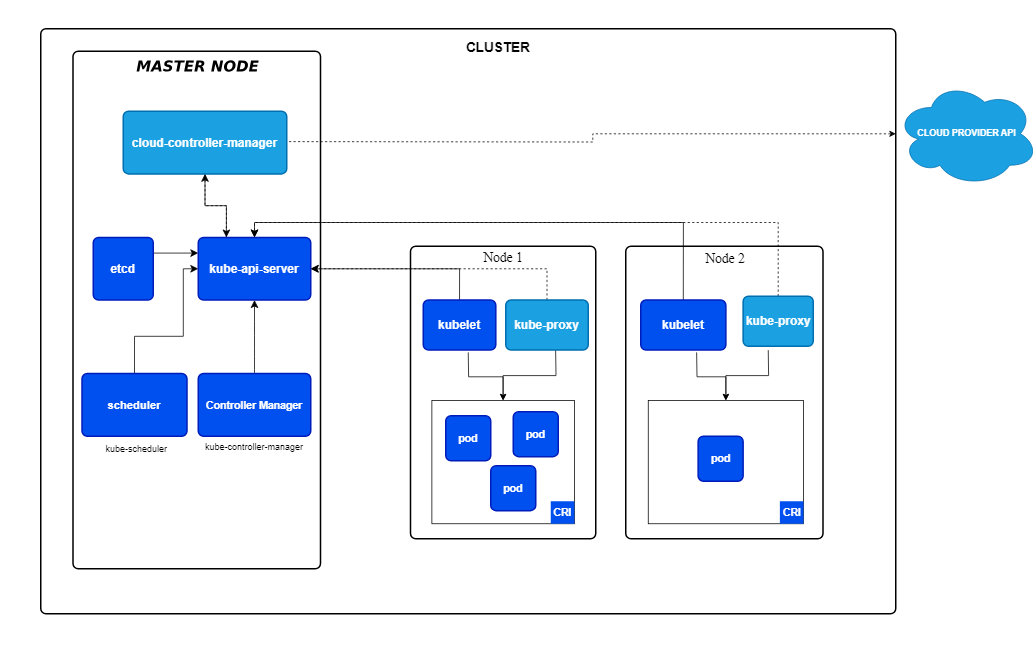
\includegraphics[scale=0.4]{img/8.png}
   \caption{Архитектура Kubernetes}
   \label{fig:ccg}
 \end{figure}

Эта многоуровневая архитектура обеспечивает масштабируемость, устойчивость и
управляемость распределенных систем, что является ключевым фактором в
обеспечении эффективной работы современных микросервисных приложений.

\subsection*{Планировщик Kubernetes (Kubernetes Scheduler)}

Планировщик Kubernetes (\textit{Scheduler}) играет ключевую роль в распределении
подов (\textit{Pods}) по узлам (\textit{Nodes}) кластера. Основная задача
планировщика — выбор подходящего узла для каждого нового пода на основе
доступных
ресурсов и требований пода \cite{luksa2017kubernetes}.
Работа планировщика включает следующие этапы:

\begin{enumerate}
   \item \textbf{Сбор информации (Information Gathering)}: Сбор информации о
требованиях пода, таких как ресурсы CPU и памяти, аффинность узлов и
допустимые (толерантности) узлы.
   \item \textbf{Фильтрация узлов (Node Filtering)}: Проверка узлов на
соответствие
требованиям пода.
   \item \textbf{Ранжирование узлов (Node Scoring)}: Ранжирование подходящих
узлов
на основе различных критериев, таких как общее количество ресурсов, близость к
другим важным подам или специфические политики распределения.
   \item \textbf{Выбор узла (Node Selection)}: Выбор узла с наивысшим рангом
для размещения пода.
\end{enumerate}

\subsection*{Отказоустойчивость подов (Pod Fault Tolerance)}

Отказоустойчивость в Kubernetes достигается через механизмы восстановления и
репликации подов:

\begin{itemize}
   \item \textbf{Репликация (Replication)}: Контроллеры, такие как
\textit{ReplicaSet}, гарантируют, что указанное количество копий пода всегда
запущено. Если под терпит сбой, контроллер автоматически создает новый под для
замены.
   \item \textbf{Самовосстанавливающиеся процессы (Self-Healing Processes)}:
Если узел
становится недоступным, планировщик Kubernetes перераспределяет поды этого узла
на другие доступные узлы.
   \item \textbf{Стратегии развертывания (Deployment Strategies)}: Механизмы,
такие как \textit{Rolling Update} в объектах \textit{Deployment}, обеспечивают
постоянное обновление подов без простоя.
\end{itemize}

\subsection*{Жизненный цикл подов (Pod Lifecycle)}

Жизненный цикл подов в Kubernetes включает следующие этапы:

\begin{enumerate}
   \item \textbf{Создание пода (Pod Creation)}: Пользователь или контроллер
создает объект пода, и API сервер записывает его в etcd.
   \item \textbf{Планирование (Scheduling)}: Планировщик Kubernetes выбирает
подходящий узел для пода.
   \item \textbf{Запуск (Launching)}: Kubelet на назначенном узле запускает
контейнеры внутри пода, используя указанную контейнерную среду выполнения.
   \item \textbf{Работа (Running)}: Под остается в рабочем состоянии, пока он
выполняет свои функции. Контроллеры наблюдают за его состоянием и
восстанавливают его при сбоях.
   \item \textbf{Удаление (Termination)}: После остановки пода (через API
сервер) Kubelet удаляет под с узла.
\end{enumerate}

Эти механизмы обеспечивают эффективное распределение и управление ресурсами, а
также повышают устойчивость и надежность работы кластера Kubernetes.

\section*{Обзор виртуальных машин в Yandex Cloud и Rustack}

В современных облачных вычислениях виртуальные машины (VM) играют ключевую роль,
обеспечивая гибкость и масштабируемость ресурсов. Yandex Cloud и Rustack
предлагают передовые решения в этой области, применяя различные подходы и
технологии.

\textbf{Yandex Cloud} \cite{yandexcloud} использует виртуализацию на уровне
гипервизора для
развертывания VM. Это обеспечивает высокую изоляцию и безопасность каждой VM,
позволяя пользователям настраивать свои экземпляры в соответствии с
индивидуальными требованиями. Yandex Cloud предлагает широкий спектр настроек
VM, включая различные конфигурации процессора, памяти и хранилища. Сетевая
инфраструктура Yandex Cloud обеспечивает высокопроизводительное подключение и
безопасность, включая виртуальные частные сети (VPN), балансировщики нагрузки и
защиту от DDoS-атак.

\textbf{Rustack} \cite{rustack}, с другой стороны, фокусируется на
предоставлении
более гибких
и настраиваемых решений в области облачных вычислений. Платформа позволяет
пользователям создавать VM с высокой степенью контроля над конфигурацией и
управлением ресурсами. Rustack поддерживает интеграцию с различными облачными и
физическими сетями, предоставляя эффективные средства для настройки сетевой
инфраструктуры, включая продвинутые опции маршрутизации и брандмауэра.

Оба провайдера поддерживают автоматизацию и оркестрацию с помощью API и
инструментов управления инфраструктурой, таких как Terraform и Ansible, что
позволяет эффективно масштабировать и управлять ресурсами. Интеграция с
современными инструментами разработки и CI/CD обеспечивает плавную интеграцию VM
в процессы разработки и развертывания.

В заключение, Yandex Cloud и Rustack предлагают разнообразные возможности для
работы с виртуальными машинами, каждый со своими уникальными преимуществами, что
делает их подходящими для различных сценариев использования в области облачных
вычислений.

\section{Выводы}

В данной главе проанализированы инструменты развертывания контейнеризированных
сред и их интеграция с Terraform и Scala. Выделены ключевые преимущества Scala,
включая статическую типизацию, мощные возможности абстракции и поддержку
функционального
программирования. Terraform оценен как мощный инструмент для управления облачной
инфраструктурой, предлагающий гибкость, контроль и возможности интеграции. 
Kubernetes рассмотрен с точки зрения типизации ресурсов и управления
контейнеризированными приложениями, подчеркивая его мощную и гибкую систему
типов.
Исследованы возможности интеграции Kubernetes и Terraform, подчеркивая потенциал
автоматизации и вызовы согласованности, а также рассмотрена роль формальных
методов
в моделировании и верификации оркестрации ресурсов. Подчеркнута значимость
формальных методов
для моделирования ресурсов IaaS, обеспечивая корректность, эффективность и
безопасность.
Проведено сравнение k3s, Kubernetes и Minikube, выделяя их применение в
различных
сценариях в зависимости от требований и ресурсов, а также учитывая результаты
оценки
производительности легковесных подходов к виртуализации. Представлен обзор
архитектуры
Kubernetes, включая компоненты управления, рабочие узлы, объекты, планировщик и 
жизненный цикл подов. Наконец, Yandex Cloud и Rustack представлены как гибкие
решения для работы с виртуальными машинами в области облачных вычислений, 
предлагая различные подходы и технологии.

\section{Постановка задачи курсового проекта}

Целью данного курсового проекта является апробация системы автомасштабирования
кластера Kubernetes на платформе Яндекс Облако. В рамках проекта
предполагается выполнение следующих ключевых задач:

\begin{enumerate}
 \item \textbf{Изучение Механизмов Автомасштабирования Kubernetes:} Детальный
анализ существующих механизмов автомасштабирования в Kubernetes, включая
изучение алгоритмов \cite{senjab2023survey}, политик и стратегий масштабирования
\cite{tran2022survey, qu2018auto, millnert2020holoscale}.
 
 \item \textbf{Настройка Платформы:} Настройка Яндекс Облако для развертывания кластера Kubernetes и
настройка соответствующей инфраструктуры. При этом будут учитываться особенности
оркестрации контейнеров с экономически эффективным автомасштабированием в
облачных средах
\cite{rodriguez2020container}.
 
 \item \textbf{Реализация и Интеграция Системы Автомасштабирования:} Разработка
системы автомасштабирования с учетом требований к эффективности распределения
ресурсов
\cite{zhong2020cost} и возможности работы в мультиоблачной среде
\cite{jiang2020cloud},
её интеграция с кластером Kubernetes на выбранной
платформе, настройка метрик и пороговых значений для масштабирования.
 
 \item \textbf{Экспериментальное Тестирование:} Проведение экспериментов для
оценки эффективности системы автомасштабирования, включая моделирование
различных сценариев нагрузки и мониторинг ресурсов с использованием подходов, 
основанных на журналировании \cite{agrawal2018log}.
 
 \item \textbf{Анализ Результатов и Оптимизация:} Анализ данных
экспериментального тестирования и внесение корректировок для улучшения
эффективности и надежности системы.
 
 \item \textbf{Оценка Применимости и Эффективности:} Оценка применимости и
эффективности реализованной системы автомасштабирования в контексте реальных
рабочих нагрузок на платформе Яндекс Облако.
\end{enumerate}

В результате выполнения проекта ожидается получение эффективной системы
автомасштабирования для кластеров Kubernetes, способной адаптироваться к
изменениям в рабочей нагрузке и обеспечивающей оптимальное использование
ресурсов на выбранных облачных платформах.

\clearpage

\chapter{Разработка алгебраического описания для представления
определений Terraform}

В работе Shapkin (2022) представлен подход, основанный на использовании
аппликативных вычислительных систем и абстрактных алгебраических структур,
для автоматизации задачи построения кода развертывания и инициализации
многокомпонентных программных систем \cite{shapkin-automation-2022}.
В этом контексте, Terraform представляет собой ключевой инструмент,
позволяющий декларативно описывать инфраструктуру как код (IaC)
\cite{iaas2017}. Однако, для эффективного использования Terraform
в рамках предложенного подхода, необходимо разработать алгебраическое
описание для представления его определений.

\section{Определение основных типов и структур данных}

Введем основные типы и структуры данных, которые будут использоваться в
дальнейшем. Это важный шаг, который позволяет нам установить общий язык и
определить основные концепции, которые будут использоваться на протяжении всей
работы.

\begin{itemize}
\item $PT$ - ProviderType (тип провайдера), общий тип, содержащий в себе все
облачные сервисы. Это множество, состоящее из всех возможных провайдеров, с
которыми может работать Terraform. Математически это можно выразить как $PT =
\bigcup_{i=1}^{k}{PT_i}$, где $PT_i$ - конкретный провайдер, например $AWS$ или
$VK$ или $Yandex$. Это ключевой тип, который определяет, с какими облачными
сервисами мы можем работать.

\item $TR$ - TerraformResource, который содержит в себе все ресурсы, которые
можно создать в HCL конфиге. Это множество, состоящее из всех возможных
ресурсов, которые можно создать при помощи Terraform. Математически это можно
выразить как $TR = \bigcup_{i=1}^{k}{TR_i}$, где $TR_i$ - конкретный ресурс.
Этот тип представляет собой основу для создания конкретных ресурсов в Terraform.

\item $IR[PT]$ - InfrastructureResource (ресурс инфраструктуры) - совокупность
всех resources и datasources, которые можно создать в HCL конфиге для данного
провайдера. Это множество, которое включает в себя все возможные ресурсы и
источники данных, которые можно создать для конкретного провайдера.
Математически это можно выразить как $IR[A] = \bigcup_{i=1}^{k}{R_i[A]} \cup
\bigcup_{i=1}^{k}{D_i[A]}$, где $R_i$ - resource, $D_i$ - datasource, $A \in
PT$. Этот тип представляет собой совокупность всех ресурсов и источников данных,
которые доступны для использования в конкретном облачном сервисе.

\item $PS[PT]$ - ProviderSettings (настройки провайдера) - тип, характеризующий
настройки провайдера, которые можно задать в HCL конфиге. Это множество, которое
включает в себя все возможные настройки, которые можно задать для конкретного
провайдера. Этот тип позволяет нам управлять настройками провайдера и
адаптировать их под конкретные требования и условия использования.

\item $BR$ - BackendResource (ресурс бэкенда) - совокупность всех ресурсов,
которые можно создать в HCL конфиге для бэкенда. Это множество, которое включает
в себя все возможные ресурсы, которые можно создать для бэкенда. Математически
это можно выразить как $BR = LB \cup RB$, где $LB$ - LocalBackend, $RB$ -
RemoteBackend. Этот тип позволяет нам управлять ресурсами бэкенда и адаптировать
их под конкретные требования и условия использования.

\item $IV$, $LV$, $OV$ - InputVariable, LocalVariable, OutputVariable -
переменные, которые можно задать в HCL конфиге. Это множества, которые включают
в себя все возможные входные, локальные и выходные переменные, которые можно
использовать в конфигурации Terraform. Эти типы позволяют нам управлять
переменными, которые используются в конфигурации, и адаптировать их под
конкретные требования и условия использования.

\item $PC$ - ProviderConfig (конфиг провайдера) - тип, который содержит в себе
все возможные ресурсы, которые можно создать в HCL конфиге для данного
провайдера, а также все возможные настройки провайдера, все возможные бэкенды,
все возможные переменные. Это множество, которое включает в себя все возможные
конфигурации, которые можно создать для каждого провайдера. Математически это
можно выразить как $PC = \bigcup_i^k{PC_i[A, T1, T2, T3]}$, где $A \in PT$, $T1
\in PS[A]$, $T2 \in BR$, $T3 \in IR[A]$. Тип $PC_i$ - конкретный конфиг
провайдера, например $PC_{AWS}$ или $PC_{VK}$ или $PC_{Yandex}$. Этот тип
представляет собой комплексный конфигурационный объект, который включает в себя
все возможные ресурсы, настройки и переменные для конкретного провайдера.
\end{itemize}

Таким образом, мы ввели типы, которые позволяют описать все возможные конфиги
для всех возможных провайдеров. Эти типы и структуры данных обеспечивают основу
для нашей работы с Terraform, позволяя нам формализовать и структурировать
данные, которые мы используем.

\section{Разработка функций для обработки определений Terraform}

В контексте нашей работы с Terraform, одним из ключевых аспектов является
создание и управление определениями, которые описывают желаемую инфраструктуру.
Это включает в себя все, от определения облачных провайдеров и настроек до
ресурсов и переменных, которые используются в конфигурации. Для того чтобы
облегчить этот процесс и сделать его более управляемым, мы вводим ряд функций,
которые позволяют нам создавать эти определения и извлекать из них информацию.

\begin{itemize}
\item $f_{PC_i}[A, T_1, T_2, T_3]:$

$T_1 \times Option[T_2] \times List[T_3] \times List[IV] \times List[LV] \times
List[OV] \rightarrow PC_i[A, T_1, T_2, T_3]$, где $A \in PT$, $T_1 \in PS[A]$,
$T_2 \in BR$, $T_3 \in IR[A]$.

Это функция для создания объектов типа $PC_i[A, T_1, T_2, T_3]$. Она принимает
на вход набор параметров, которые описывают конкретный конфиг провайдера, и
возвращает объект этого типа. Эта функция играет важную роль в нашей системе,
поскольку она позволяет нам создавать конкретные конфиги провайдера на основе
заданных параметров, что обеспечивает большую гибкость и контроль над процессом
создания конфигураций.

\item $to_{HCL}$ - функция, которая преобразует объект типа $TR$ в HCL конфиг (в
его строковое представление).

$to_{HCL}: TR \rightarrow String$.

Эта функция преобразует объект типа $TR$ в его строковое представление в формате
HCL. Это ключевой элемент нашей системы, поскольку он позволяет нам генерировать
конфигурационные файлы Terraform на основе наших объектов типа $TR$. Это
обеспечивает большую гибкость и контроль над процессом создания конфигураций,
поскольку мы можем легко преобразовать наши объекты в конфигурационные файлы.

\item $to_{HCL}(PC[A, T_1, T_2, T_3])$ - функция, которая возвращает HCL конфиг
в строковом виде для типа $PC[A, T_1, T_2, T_3]$:

\begin{align*}
  to_{HCL}(PC[A, T1, T2, T3]) = \{ \\
  &allResources = Concatenate( \\
  &\quad provider, \\
  &\quad backend, \\
  &\quad resources, \\
  &\quad inputVars, \\
  &\quad localVars, \\
  &\quad outputVars \\
  &), \\
  &resourceStrings = Map(allResources, \\
  &resource \rightarrow to_{HCL}(resource)), \\
  &hcl = Join(resourceStrings, "\backslash n \backslash n") \\
  &\} \rightarrow hcl
\end{align*}

Эта функция преобразует объект типа $PC[A, T_1, T_2, T_3]$ в его строковое
представление в формате HCL. Это обеспечивает еще один уровень гибкости и
контроля над процессом создания конфигураций, поскольку мы можем легко
преобразовать наши объекты в конфигурационные файлы.

\end{itemize}

Введение этих функций является важным шагом в нашей работе с Terraform. Они
обеспечивают нам необходимые инструменты для создания и управления
конфигурациями Terraform, что в свою очередь позволяет нам более эффективно и
надежно управлять нашей инфраструктурой.

В дополнение к этим функциям, мы также используем ряд операций, которые помогают
нам обрабатывать и управлять нашими данными:

\begin{itemize}
\item $Concatenate$ - Функция, которая объединяет несколько списков в один.
Backend рассматривается как список, который может содержать ноль или один
элемент. Это позволяет нам объединять различные ресурсы и переменные в один
общий список, который затем можно использовать для генерации конфигурационного
файла Terraform.

\item $Map$ - Функция, которая применяет функцию (в данном случае, $to_{HCL}$) к
каждому элементу списка и возвращает список результатов. Это позволяет нам
преобразовать каждый ресурс или переменную в его строковое представление в
формате HCL.

\item $Join$ - Функция, которая объединяет все строки в списке в одну строку, с
разделительной строкой (в данном случае, "$\backslash$ n$\backslash$ n") между
каждым элементом. Это позволяет нам объединять все строковые представления
ресурсов и переменных в один общий конфигурационный файл Terraform.
\end{itemize}

Вместе эти функции и операции образуют мощный инструментарий для работы с
\newline
Terraform, обеспечивая нам необходимую гибкость и контроль для создания и
управления конфигурациями. Они позволяют нам
эффективно описывать и изменять нашу инфраструктуру, а также обеспечивают
надежность и безопасность нашего процесса управления инфраструктурой.


\section{Разработка функций для инкапсуляции процесса развертывания определений
Terraform}


После того как мы определили основные типы данных и функции для создания и
преобразования определений Terraform, следующим шагом является разработка
функций, которые инкапсулируют процесс развертывания этих определений. Эти
функции обеспечивают автоматизацию и упрощение процесса развертывания, позволяя
нам легко и надежно развертывать наши конфигурации Terraform.

Одной из ключевых функций, которую мы разрабатываем, является функция $deploy$,
которая принимает на вход конфигурацию провайдера $PC[A, T_1, T_2, T_3]$ и
выполняет все необходимые действия для развертывания этой конфигурации. Это
включает в себя генерацию HCL конфигурации, инициализацию Terraform, применение
конфигурации и, при необходимости, уничтожение существующей инфраструктуры.

$$
deploy: PC[A, T_1, T_2, T_3] \rightarrow State
$$

Здесь $State$ - это тип, который представляет состояние развертывания, включая
информацию о развернутых ресурсах, статусе развертывания и возможных ошибках.

Функция $deploy$ использует функцию $to_{HCL}$ для генерации HCL конфигурации из
объекта $PC[A, T_1, T_2, T_3]$. Затем она инициализирует Terraform с
использованием этой конфигурации и применяет ее, развертывая ресурсы в
соответствии с конфигурацией. Если указано, функция также может уничтожить
существующую инфраструктуру перед развертыванием новой.

Важно отметить, что функция $deploy$ обеспечивает управление состоянием
развертывания, что позволяет нам отслеживать прогресс развертывания и
обрабатывать возможные ошибки. Это обеспечивает большую надежность и
контролируемость процесса развертывания.

В дополнение к функции $deploy$, мы также разрабатываем ряд вспомогательных
функций, которые обеспечивают дополнительные возможности управления
развертыванием. Например, мы можем разработать функции для проверки статуса
развертывания, получения информации о развернутых ресурсах, или выполнения
других действий, связанных с управлением развертыванием.

\section{Выводы}

В ходе разработки алгебраического описания для представления определений
Terraform был проведен анализ основных типов и структур данных, используемых в
Terraform. Были введены типы, такие как ProviderType, TerraformResource,
InfrastructureResource, \newline ProviderSettings, BackendResource, и
ProviderConfig,
которые позволяют описать все возможные конфигурации для всех возможных
провайдеров.

Были разработаны функции для создания этих типов, а также функции для
преобразования этих типов в HCL конфигурации. Это позволяет нам автоматизировать
и упростить процесс создания конфигураций Terraform, обеспечивая большую
гибкость и контроль над этим процессом.

Также были разработаны функции для инкапсуляции процесса развертывания
определений Terraform. Эти функции позволяют нам автоматизировать и упростить
процесс развертывания, обеспечивая надежность и контролируемость этого процесса.

В целом, разработанные типы данных, функции и операции образуют мощный
инструментарий для работы с Terraform, обеспечивая необходимую гибкость и
контроль для создания и управления конфигурациями Terraform. Это позволяет нам
эффективно описывать и изменять нашу инфраструктуру, а также обеспечивает
надежность и безопасность нашего процесса управления инфраструктурой.

\clearpage

\chapter{Результаты проектирования архитектуры модуля для оркестрации
Kubernetes}


\section{Описание архитектуры модуля для развертывания Terraform}

В данном разделе представлено описание архитектуры модулей, которые включают в
себя "Case Classes Generator", "HCL Generator", "HCL Deployer", "Autoscaler" и
"Config Parser". Эти модули взаимодействуют друг с другом для обеспечения
функциональности приложения.

\subsection{Case Classes Generator}

Первый модуль, "Case Classes Generator" (см. Рисунок \ref{fig:ccg}), отвечает за
получение метаданных и формирование case classes. Этот модуль принимает на вход
данные от "Plugin Analyzer" и "Docs Analyzer", которые анализируют плагины и
документацию соответственно. Результатом работы этого модуля являются
сгенерированные case classes, которые затем передаются в "HCL Generator".

\begin{figure}[h]
  \centering
  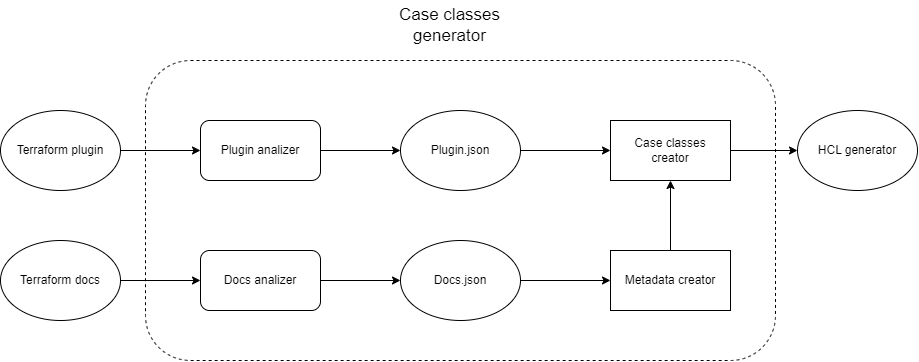
\includegraphics[scale=0.5]{img/1.png}
  \caption{Архитектура модуля "Case Classes Generator"}
  \label{fig:ccg}
\end{figure}

\subsection{HCL Generator}

"HCL Generator" (см. Рисунок \ref{fig:hclg}) является вторым модулем и не имеет
собственной точки входа. Он получает case classes от "Case Classes Generator" и
генерирует из них HCL конфигурацию. Этот модуль является ключевым для получения
HCL конфига и его последующего запуска.

\begin{figure}[h]
  \centering
  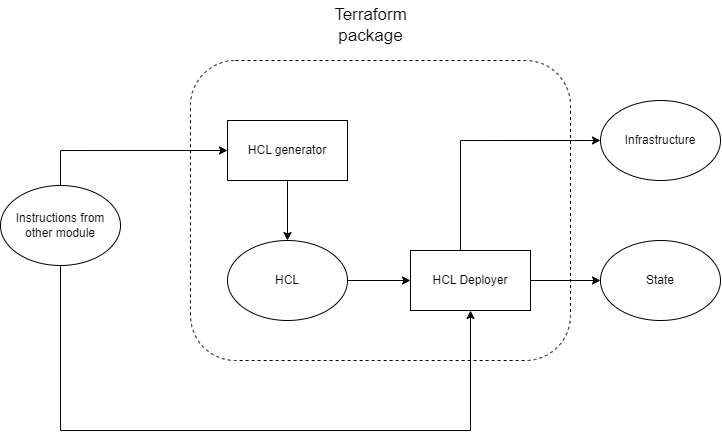
\includegraphics[scale=0.6]{img/2.png}
  \caption{Архитектура модуля "HCL Generator"}
  \label{fig:hclg}
\end{figure}

\subsection{HCL Deployer и Autoscaler}

Третий модуль, "HCL Deployer" (см. Рисунок \ref{fig:hdas}), использует HCL
конфигурацию, сгенерированную "HCL Generator", для изменения архитектуры
кластера. Он также подключается к API Kubernetes для получения состояния
кластера и принятия решений о масштабировании, а также перемещения pods с одной
node на другую. Этот модуль завернут в Helm chart и его следует запускать на
master node кластера для автоматического масштабирования кластера.

\begin{figure}[h]
  \centering
  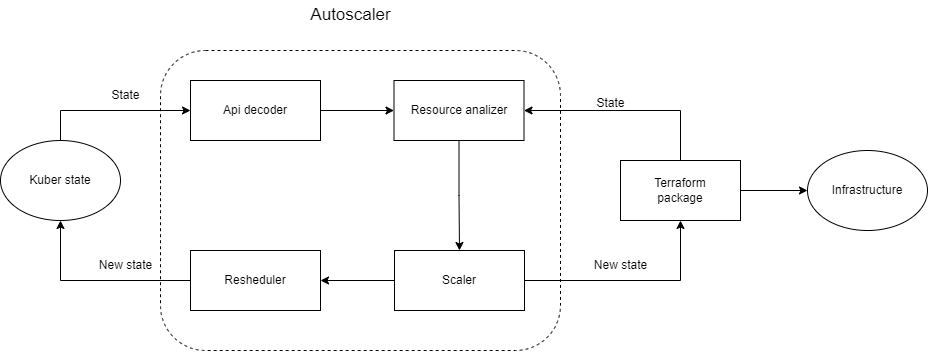
\includegraphics[scale=0.5]{img/3.png}
  \caption{Архитектура модулей "HCL Deployer" и "Autoscaler"}
  \label{fig:hdas}
\end{figure}

\vspace{15mm}

\subsection{Config Parser}

Четвертый модуль, "Config Parser" (см. Рисунок \ref{fig:cp}), использует HCL
конфигурацию для развертывания кластера с запущенным на нем модулем "HCL
Deployer", а также для первичной настройки модуля "HCL Deployer" и архитектуры
кластера. 

\begin{figure}[h]
  \centering
  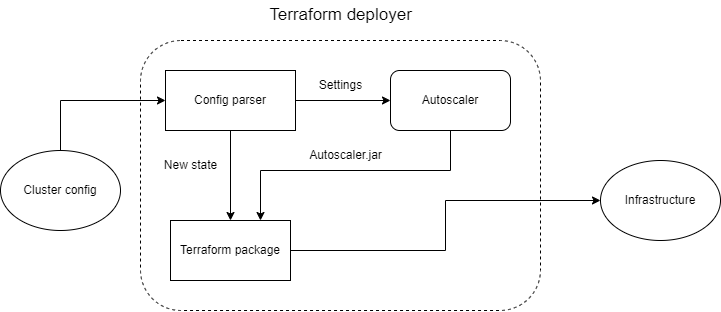
\includegraphics[scale=0.6]{img/4.png}
  \caption{Архитектура модуля "Config Parser"}
  \label{fig:cp}
\end{figure}

\section{Разработка интерфейсов и классов модуля для генерации HCL конфигурации}

В процессе разработки модуля-обертки для развертывания типизированных
определений Terraform, было необходимо создать ряд интерфейсов и классов,
которые обеспечивают структуру и функциональность модуля. Эти интерфейсы и
классы были разработаны с учетом особенностей работы Terraform и требований к
типизации и структуре данных.

В основе архитектуры модуля лежат следующие интерфейсы и классы:

\begin{itemize}
\item $ProviderType$: Этот интерфейс представляет тип провайдера в
Terraform. Он служит базовым интерфейсом для всех конкретных типов провайдеров.

\item $TerraformResource$: Этот абстрактный класс представляет ресурс в
Terraform. Он содержит метод $toHCL$, который должен быть реализован в
каждом конкретном классе ресурса для преобразования объекта ресурса в его HCL
представление.

\item $InfrastructureResource[T <: ProviderType]$: Этот интерфейс
расширяет \newline $TerraformResource$ и представляет ресурс инфраструктуры в
Terraform. Он параметризован типом провайдера.

\item $ProviderSettings[T <: ProviderType]$: Этот интерфейс расширяет
\newline $TerraformResource$ и представляет настройки провайдера в Terraform.
Он также параметризован типом провайдера.

\item $BackendResource$: Этот интерфейс расширяет
$TerraformResource$ и представляет ресурс бэкенда в Terraform.

\item $ProviderConfig[A, T_1, T_2, T_3]$: 
$A <: ProviderType, T_1 <: ProviderSettings[A], T_2 <:
BackendResource, T_3 <: InfrastructureResource[A]$. 
Этот класс представляет конфигурацию провайдера в Terraform.
Он содержит все необходимые данные для создания и развертывания
конфигурации провайдера, включая настройки провайдера,
ресурс бэкенда и ресурсы инфраструктуры. Он также содержит метод $toHCL$
для преобразования конфигурации провайдера в его HCL представление.
\end{itemize}

Для успешного проектирования модуля было необходимо разработать механизмы для
извлечения информации о структуре определений ресурсов и источников данных из
Terraform. Это было достигнуто путем создания специальных компонентов, которые
выполняют следующие функции:

\begin{itemize}
  \item Получение структуры ресурсов из определения плагина Terraform:
Этот компонент отвечает за анализ определений плагина Terraform, написанных на
языке Go, и извлечение из них структуры ресурсов. Это включает в себя информацию
о типах ресурсов, их свойствах и связях между ними.
  
  \item Анализ документации и получение из нее полезной информации:
Этот компонент отвечает за анализ документации Terraform и извлечение из нее
полезной информации. Это может включать в себя дополнительные свойства полей,
которые не могут быть получены из анализа определений плагина, такие как
возможность содержания полем типа JSON или ID.
  
  \item Преобразование полученных данных в формат JSON: После
извлечения информации о структуре ресурсов и анализа документации, эта
информация преобразуется в формат JSON для дальнейшего использования. Это
включает в себя создание двух файлов JSON, каждый из которых содержит информацию
о структуре ресурсов и источников данных.
  
  \item Передача полученных данных в основной модуль на Scala: После
преобразования данных в формат JSON, они передаются в основной модуль на Scala.
Этот модуль затем использует эти данные для создания case classes, с
определенной на них функцией toHCL, которые представляют собой типизированные
определения Terraform.
\end{itemize}

\section{Разработка функций для взаимодействия с Kubernetes}

\subsection{Общее описание функций и типов модуля}

Для взаимодействия с Kubernetes необходимо разработать следующие типы, которые
будут хранить конфигурацию всего кластера:

\begin{itemize}
\item \textbf{Node}: Этот тип представляет собой узел в кластере Kubernetes.
Узел может быть виртуальной или физической машиной в зависимости от кластера.
\item \textbf{Pod}: Pod в Kubernetes - это наименьшая и простейшая единица в
модели объектов Kubernetes, которую создает или развертывает пользователь. Pod
представляет собой группу одного или нескольких контейнеров, которые разделяют
хранилище и сетевые ресурсы, и спецификация о том, как запускать контейнеры.
\item \textbf{Event}: События в Kubernetes представляют собой объекты, которые
предоставляют представление о том, что происходит внутри кластера, например,
какие поды/узлы были запущены/остановлены и т.д.
\item \textbf{KuberInfo}: Этот тип представляет собой общую информацию о
кластере Kubernetes, такую как количество узлов, подов, событий и т.д.
\end{itemize}

Также необходимо разработать следующие функции:

\begin{itemize}
\item \textbf{drainNodes}: Функция для удаления подов с узлов.
\item \textbf{processResources}: Функция для обработки ресурсов в Kubernetes.
\item \textbf{increaseReplicas}: Функция для увеличения количества реплик в
ресурсе.
\item \textbf{cordonNode}: Функция для установки узла в режим "не планируемый",
что означает, что на него не будут назначены новые поды.
\item \textbf{getResources}: Функция для получения списка всех ресурсов в
кластере.
\item \textbf{getAutoscaler}: Функция для получения информации об
автомасштабировании для определенного развертывания.
\item \textbf{disableAutoscaler}: Функция для отключения автомасштабирования для
определенного развертывания.
\item \textbf{enableAutoscaler}: Функция для включения автомасштабирования для
определенного развертывания.
\item \textbf{deletePod}: Функция для удаления пода.
\item \textbf{waitUntilAllPodsVerified}: Функция для ожидания, пока все поды не
будут проверены и не начнут работать.
\end{itemize}

Пожалуйста, обратите внимание, что все эти функции предполагают наличие
экземпляра KubernetesClient, который предоставляет методы для взаимодействия с
API Kubernetes. Эти функции используются для управления ресурсами в кластере
Kubernetes, включая узлы, поды, репликации и автомасштабирование.

Все функции возвращают результат в виде IO, что позволяет обрабатывать
асинхронные операции и ошибки в функциональном стиле.

Важно отметить, что эти функции представляют собой общий интерфейс для
взаимодействия с Kubernetes и могут быть расширены или модифицированы в
соответствии с конкретными требованиями приложения.

\subsection{Работа Scaler}

Scaler является ключевым компонентом в системе, который отвечает за
автоматическое масштабирование ресурсов в Kubernetes. Он использует информацию
из KuberInfo для определения текущего состояния кластера и принятия решений о
масштабировании.

\begin{itemize}
\item \textbf{Проверка возможности перемещения подов}: Scaler анализирует
текущее распределение подов по узлам и определяет, можно ли переместить поды
таким образом, чтобы один или несколько узлов были полностью освобождены. Это
может быть полезно для оптимизации использования ресурсов или подготовки узла к
обслуживанию или удалению. При этом Scaler учитывает ресурсы, необходимые для
поддержания работоспособности каждого пода, чтобы гарантировать, что после
перемещения все поды смогут корректно функционировать.

\item \textbf{Проверка наличия достаточных ресурсов}: Scaler также проверяет,
нет ли ситуации, когда под не может быть запущен из-за нехватки ресурсов. Это
может произойти, если все узлы в кластере загружены или если под требует больше
ресурсов, чем доступно на любом из узлов. В таком случае Scaler может принять
решение о масштабировании узлов, чтобы обеспечить достаточность ресурсов для
всех подов.
\end{itemize}

Важно отметить, что действия Scaler зависят от конкретной политики
масштабирования, которая может варьироваться в зависимости от требований
приложения и конфигурации кластера. Например, некоторые системы могут
предпочитать минимизировать количество используемых узлов для снижения затрат, в
то время как другие могут стремиться максимизировать распределение нагрузки для
повышения отказоустойчивости.

\section{Разработка функций для взаимодействия с Terraform и Kubernetes}

Для эффективного взаимодействия между Terraform и Kubernetes необходимо
установить соответствие между серверами, объявленными в Terraform, и узлами
(Nodes) в Kubernetes. Это соответствие, или биекция, позволяет нам управлять и
изменять конфигурацию обоих систем согласованно.

\subsection{Установление биекции}

Биекция между серверами Terraform и узлами Kubernetes позволяет нам точно знать,
какой сервер Terraform соответствует какому узлу Kubernetes. Это важно,
поскольку обе системы имеют разные представления об инфраструктуре и управляют
ею по-разному. Установление такого соответствия позволяет нам синхронизировать
состояние обоих систем.

Для установления этого соответствия мы вводим специальные теги при создании
серверов в конфигурации Terraform. Эти теги позволяют нам однозначно
идентифицировать каждый сервер и узел, обеспечивая точное соответствие между
ними.

Важно отметить, что все эти операции должны быть автоматизированы и
синхронизированы, чтобы обеспечить согласованность и надежность нашей
инфраструктуры. Это может потребовать разработки дополнительных функций или
скриптов, которые будут отслеживать состояние обоих систем и автоматически
применять необходимые изменения при обнаружении отклонений от желаемого
состояния.

\section{Выводы}

В ходе проектирования архитектуры модуля-обертки для развертывания
типизированных определений Terraform были разработаны и описаны ключевые
компоненты системы, включая "Case Classes Generator", "HCL Generator", "HCL
Deployer", "Autoscaler" и "Config Parser". Эти модули взаимодействуют друг с
другом для обеспечения функциональности приложения, включая генерацию HCL
конфигурации, развертывание и масштабирование инфраструктуры, а также анализ и
обработку конфигурации.

Были разработаны интерфейсы и классы для генерации HCL конфигурации, включая
ProviderType, TerraformResource, InfrastructureResource, ProviderSettings,
BackendResource и ProviderConfig. Эти интерфейсы и классы обеспечивают гибкость
и расширяемость системы, позволяя поддерживать различные типы провайдеров и
ресурсов.

Для взаимодействия с Kubernetes были разработаны типы Node, Pod, Event и
KuberInfo, а также функции для управления узлами и подами, масштабирования
ресурсов и анализа состояния кластера. Эти функции предоставляют общий интерфейс
для взаимодействия с Kubernetes и могут быть расширены или модифицированы в
соответствии с конкретными требованиями приложения.

Была реализована биекция между серверами Terraform и узлами Kubernetes,
позволяющая синхронизировать состояние обоих систем и управлять их конфигурацией
согласованно. Для установления этого соответствия были введены специальные теги
при создании серверов в конфигурации Terraform.

В целом, разработанная архитектура модуля-обертки для развертывания
типизированных определений Terraform обеспечивает эффективное взаимодействие
между Terraform и Kubernetes, позволяя автоматизировать процесс развертывания и
управления инфраструктурой.

\clearpage

\chapter{Реализация и экспериментальная проверка работоспособности модуля}

\section{Реализация анализатора плагинов Terraform}

Для реализации анализатора плагинов Terraform был использован язык
программирования Go, так как Terraform и большинство его плагинов написаны на
Go.

Анализатор плагинов Terraform реализован как отдельное приложение на Go, которое
анализирует исходный код плагинов Terraform и извлекает из него метаданные,
необходимые для генерации классов-оберток на Scala.

В основе анализатора лежит рефлексия - механизм, позволяющий программам
исследовать структуру кода во время выполнения. С помощью рефлексии анализатор
исследует структуру плагина Terraform, извлекает информацию о типах ресурсов и
их свойствах и преобразует эту информацию в формат, подходящий для генерации
классов-оберток на Scala.

В процессе анализа анализатор обходит все структуры и поля в плагине,
обрабатывая каждое поле в зависимости от его типа. Для структур и отображений
(map) анализатор рекурсивно обходит их поля, для срезов (slice) - их элементы.
Функции и другие необрабатываемые типы пропускаются.

Результат работы анализатора - файл JSON с метаданными плагина, который затем
используется модулем генерации классов-оберток для создания классов-оберток на
Scala.

Код анализатора находится в Приложении \ref{sec:appendix1}.

В этом коде функции обхода структур (walkStruct), обхода срезов (walkSlice) и
обхода отображений (walkMap) используются для обхода соответствующих структур
данных. Они вызывают функцию обработки значения (processValue) для каждого поля
или элемента, которая в свою очередь обрабатывает значение в зависимости от его
типа и возвращает его в формате, подходящем для записи в JSON.

Функция проверки допустимости значения (valueIsValid) используется для
определения, является ли значение обрабатываемым. Она возвращает false для
функций и других типов значений, которые не могут быть корректно преобразованы в
JSON.

В главной функции (main) происходит инициализация плагина Terraform, извлечение
информации о провайдере с помощью рефлексии, преобразование этой информации в
JSON и запись JSON в файл.

Пример файла JSON с метаданными плагина Terraform см. в Приложении
\ref{sec:appendix2}.

Таким образом, анализатор плагинов Terraform позволяет извлечь из плагинов
метаданные, необходимые для генерации классов-оберток на Scala. Эти метаданные
включают в себя информацию о типах ресурсов и их свойствах, которые затем
используются при генерации кода на Scala.

\section{Реализация анализатора документации}

Анализатор документации реализован на языке Python и использует библиотеки json,
os, re и hcl. Он проходит через все файлы в указанной директории, извлекает
блоки кода конфигурации Terraform (HCL) из файлов с расширением .md или
.markdown, анализирует их и сохраняет результат в формате JSON.

Вот основные шаги работы анализатора:

\begin{itemize}
  \item Извлечение блоков кода конфигурации Terraform из файлов документации.
Это достигается с помощью функции извлечения блоков кода из директории
(extract\_code\_blocks\_from\_directory), которая проходит через все файлы в
указанной директории и вызывает функцию извлечения блоков кода из файла
(extract\_code\_blocks\_from\_file) для каждого файла. Функция извлечения блоков
кода из файла открывает файл, читает его содержимое и использует регулярное
выражение для поиска блоков кода конфигурации Terraform.
  
  \item Анализ блоков кода конфигурации Terraform. Это делается с помощью
функции анализа конфигурации Terraform (parse\_terraform), которая принимает на
вход массив блоков кода конфигурации Terraform и пытается проанализировать
каждый из них с помощью библиотеки hcl. Если анализ проходит успешно, результат
добавляется в массив проанализированных блоков (hcl\_arr).
  
  \item Преобразование сложных структур данных в плоский формат. Это делается с
помощью функции выравнивания словаря (flatten\_dict), которая принимает на вход
словарь и преобразует его в плоский формат, где каждый ключ представляет собой
путь к соответствующему значению в исходном словаре.
  
  \item Сохранение результатов в файл. После обработки всех блоков кода
конфигурации Terraform результаты сохраняются в файл в формате JSON.
\end{itemize}

Полный код анализатора представлен в Приложении \ref{sec:appendix3}.

Пример файла JSON с метаданными документации Terraform см. в Приложении
\ref{sec:appendix4}.

\section{Реализация модуля генерации классов-оберток}

Модуль состоит из многих файлов, опишем основные из них в текущем разделе.

\subsection{Реализация анализатора документации}

Модуль анализатора документации отвечает за обработку и анализ документации в
формате JSON, полученной из Terraform. Он использует библиотеку Circe для
декодирования JSON и библиотеку Scala для работы с регулярными выражениями и
файлами.

Вот основные компоненты этого модуля:

\begin{itemize}
  \item JsonValue: это абстрактный класс, представляющий значение JSON. Он имеет
четыре подкласса: JsonString, JsonBool, JsonLong и JsonDouble, которые
представляют соответствующие типы данных JSON.

  \item JsonMap: это тип для представления отображения JSON, где ключи - это
строки, а значения - это списки значений JSON.
  
  \item DocsInfo: это класс, который содержит информацию, извлеченную из
документации. Он содержит различные отображения для хранения доменов,
IP-адресов, масок IP-адресов, строк JSON и ссылок на поля.
  
  \item decodeJsonMap: эта функция декодирует строку JSON в JsonMap. Если
происходит ошибка декодирования, она выбрасывает исключение.
  
  \item filterJsonMap: эта функция фильтрует JsonMap, оставляя только ключи,
которые начинаются с "output.", "resource." или "data.".
  
  \item definePatterns: эта функция определяет регулярные выражения для
различных типов значений, таких как поля, домены, IP-адреса и маски IP-адресов.
  
  \item decodeAndFilterJson: это основная функция модуля. Она принимает строку
JSON, декодирует ее в JsonMap, фильтрует отображение, извлекает различные типы
значений и возвращает DocsInfo с этой информацией.
\end{itemize}

\subsection{Описание классов и функций}

Основные классы представлены на рисунке \ref{fig:uml1}.

\begin{figure}[h]
  \centering
  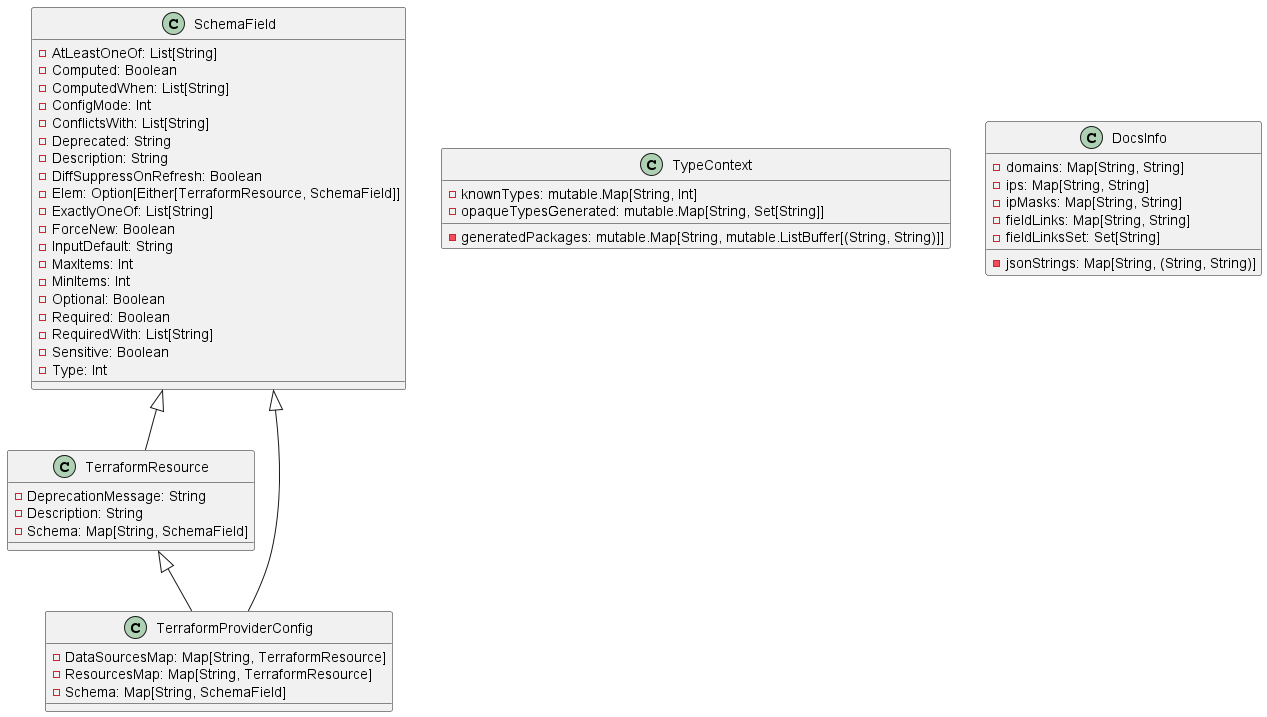
\includegraphics[scale=0.35]{img/5.png}
  \caption{Основные классы модуля генерации классов-оберток}
  \label{fig:uml1}
\end{figure}

\vspace{60mm}

Далее опишем основные классы и функции модуля:

\begin{itemize}
  \item SchemaField: Этот класс представляет собой модель для полей схемы в
Terraform. Он содержит различные атрибуты, такие как AtLeastOneOf, Computed,
ComputedWhen, ConfigMode, ConflictsWith, Deprecated, Description,
DiffSuppressOnRefresh, Elem, ExactlyOneOf, ForceNew, InputDefault, MaxItems,
MinItems, Optional, Required, RequiredWith, Sensitive, Type. Elem - это
опциональное поле, которое может содержать либо TerraformResource, либо другой
SchemaField.
  
  \item TerraformProviderConfig: Этот класс представляет конфигурацию провайдера
Terraform. Он содержит отображения для DataSourcesMap, ResourcesMap и Schema.
  
  \item TerraformResource: Этот класс представляет ресурс в Terraform. Он
содержит DeprecationMessage, Description и Schema.
  
  \item TypeContext: Этот класс содержит контекст для типов, включая knownTypes,
generatedPackages и opaqueTypesGenerated.
  
  \item DocsInfo: Этот класс содержит информацию, извлеченную из документации
Terraform. Он содержит отображения для domains, ips, ipMasks, jsonStrings,
fieldLinks и множество fieldLinksSet.
  
  \item TypeCodes: Этот объект содержит константы для различных типов полей.
  
  \item generateFieldType: Эта функция генерирует тип поля на основе
SchemaField.
  
  \item updateFieldWithType: Эта функция обновляет поле с типом на основе
SchemaField.
  
  \item generateTodoComment: Эта функция генерирует комментарий TODO для поля.
  
  \item generateSchemaForElem: Эта функция генерирует схему для элемента на
основе SchemaField.
  
  \item generateSchemaField: Эта функция генерирует поле схемы на основе
SchemaField.
  
  \item generateResourceClassName: Эта функция генерирует имя класса ресурса.
  
  \item generatePackageName: Эта функция генерирует имя пакета.
  
  \item generateFullName: Эта функция генерирует полное имя.
  
  \item generateFields: Эта функция генерирует поля для ресурса.
  
  \item getUniqueClassName: Эта функция генерирует уникальное имя класса.
  
  \item generateToHCLBody: Эта функция генерирует тело метода toHCL.
  
  \item generateToHCLMethod: Эта функция генерирует метод toHCL.
  
  \item generateFieldDescriptions: Эта функция генерирует описания полей для
ScalaDoc.
  
  \item generateClassDoc: Эта функция генерирует документацию для класса,
включая описание ресурса и описания полей.
  
  \item generateDeprecationAnnotation: Эта функция генерирует аннотацию
устаревания, если ресурс устарел.
  
  \item generateClassDef: Эта функция генерирует определение класса, включая его
поля и методы.
  
  \item generatePackageCode: Эта функция генерирует код пакета, включая
определения классов и связанных полей.
  
  \item updateContext: Эта функция обновляет контекст, добавляя новые классы и
пакеты.
  
  \item generateLinkedFields: Эта функция генерирует связанные поля для ресурса.
  
  \item generateResourceClass: Эта функция генерирует класс ресурса на основе
конфигурации ресурса.
  
  \item generateCaseClasses: Эта функция генерирует классы-обертки для
конфигурации провайдера.
  
  \item generateDataSources: Эта функция генерирует источники данных для
конфигурации провайдера.
  
  \item generateResources: Эта функция генерирует ресурсы для конфигурации
провайдера.
  
  \item generateProviderResource: Эта функция генерирует ресурс провайдера для
конфигурации провайдера.
  
  \item printFieldLinksInfo: Эта функция выводит информацию о связанных полях.
  
  \item generatePackages: Эта функция генерирует пакеты на основе контекста.
  
  \item generateProviderPackage: Эта функция генерирует пакет провайдера.
\end{itemize}

Код для данного модуля не будет приведен в текущей статье из-за его большого
объема. Полный код доступен в репозитории проекта.

\subsection{Пример работы}

В этом примере мы используем библиотеку Circe для декодирования JSON,
представляющего конфигурацию провайдера Terraform, и генерируем соответствующие
классы Scala.

Сначала мы читаем JSON из файла и декодируем его в объект
TerraformProviderConfig. Затем мы генерируем классы Scala для каждого ресурса и
источника данных в конфигурации провайдера с использованием функции
generateCaseClasses. Наконец, мы записываем сгенерированный код Scala в файлы в
соответствующих пакетах.

Пример кода см. в Приложении \ref{sec:appendix6}.

Диаграмма классов для сгенерированного кода Scala представлена на рисунке
\ref{fig:uml2}.

\begin{figure}[h]
  \centering
  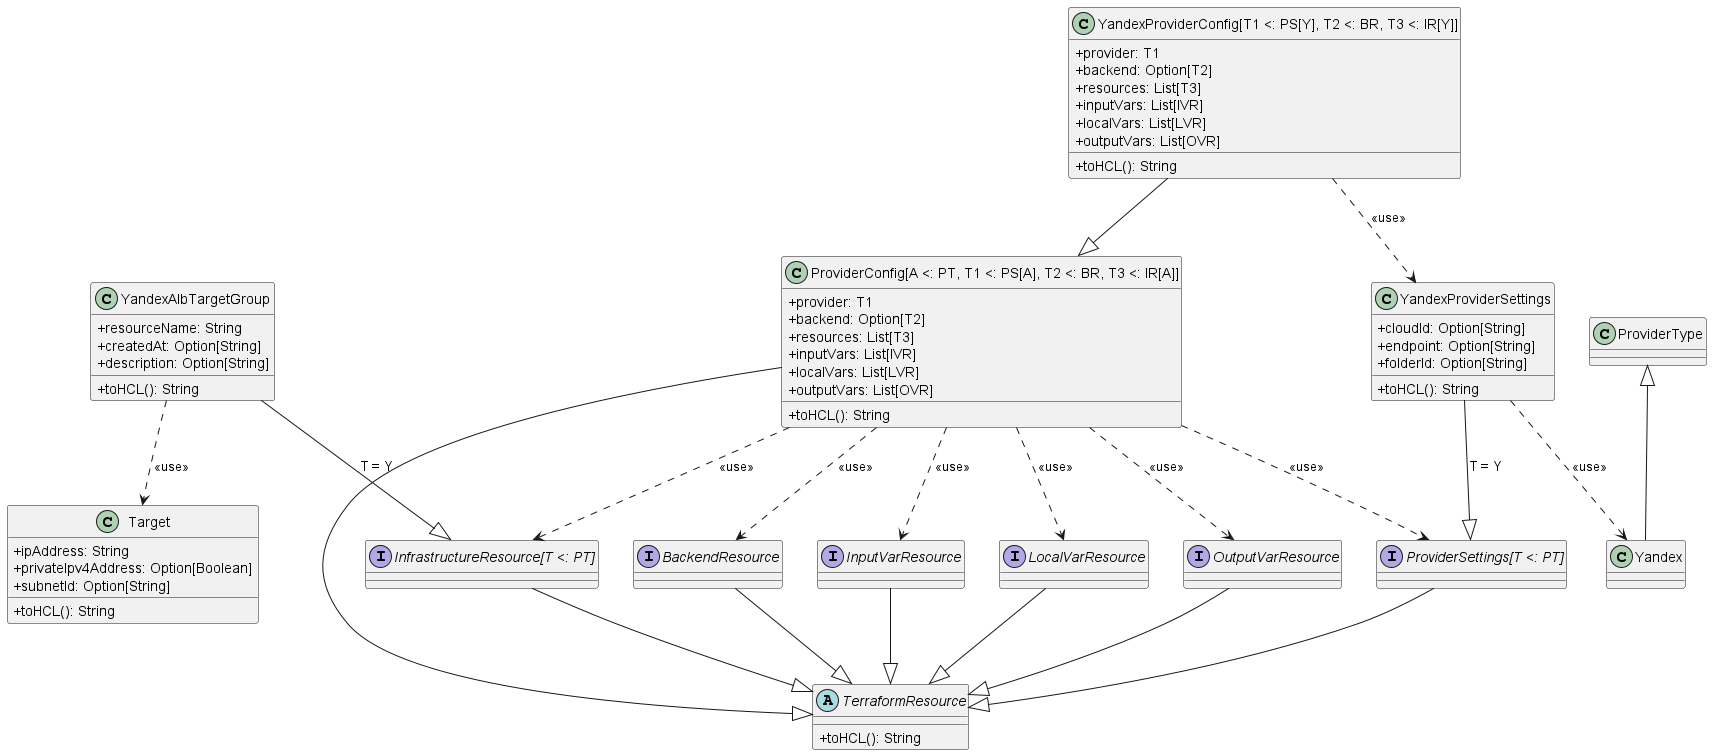
\includegraphics[scale=0.25]{img/6.png}
  \caption{Диаграмма классов для сгенерированного кода Scala}
  \label{fig:uml2}
\end{figure}

В этом примере мы используем файлы JSON, сгенерированные с помощью инструментов
извлечения документации Terraform и преобразования конфигурации Terraform в
JSON, для представления конфигурации провайдера Terraform и связанных с ним
документов. Эти файлы затем используются для генерации классов Scala, которые
могут быть использованы для работы с этим провайдером в Scala.

\section{Реализация модуля для работы с программным интерфейсом Kubernetes}

\subsection{Описание классов}

В данном модуле определены следующие классы:
\begin{itemize}
  \item AllocatedResources: Этот класс представляет выделенные ресурсы. Он
содержит следующие поля: cpuRequests (запросы процессорного времени), cpuLimits
(ограничения процессорного времени), memoryRequests (запросы памяти),
memoryLimits (ограничения памяти), ephemeralStorageRequests (запросы эфемерного
хранилища), ephemeralStorageLimits (ограничения эфемерного хранилища),
hugepages2MiRequests (запросы огромных страниц размером 2 Ми),
hugepages2MiLimits (ограничения огромных страниц размером 2 Ми),
hugepages1GiRequests (запросы огромных страниц размером 1 Ги),
hugepages1GiLimits (ограничения огромных страниц размером 1 Ги). Все поля имеют
тип BigDecimal.
  
  \item ContainerStates: Этот класс представляет состояния контейнера. Он
содержит одно поле: id (идентификатор) типа String.
  
  \item PodConditions: Этот класс представляет условия модуля (пода). Он
содержит следующие поля: conditionType (тип условия) типа String и status
(статус) типа Boolean.
  
  \item MyPod: Этот класс представляет модуль (под). Он содержит следующие поля:
ip (IP-адрес) типа Option[String], name (имя) типа String, status (статус) типа
Option[String], startedAt (время запуска) типа Option[String], createdAt (время
создания) типа Option[String], age (возраст) типа Option[String], ageInSec
(возраст в секундах) типа Long, restarts (перезапуски) типа Int, states
(состояния) типа List[ContainerStates], allocatedResources (выделенные ресурсы)
типа AllocatedResources, namespace (пространство имен) типа String, isSystem
(системный) типа Boolean, failedScheduling (не удалось запланировать) типа
Boolean, events (события) типа Map[String, MyEvent], conditions (условия) типа
List[PodConditions], uid (уникальный идентификатор) типа String.
  
  \item MyNode: Этот класс представляет узел. Он содержит следующие поля: name
(имя) типа String, status (статус) типа Map[String, Boolean], pods (модули) типа
Map[String, MyPod], ip (IP-адреса) типа Map[String, String], allocatedResources
(выделенные ресурсы) типа AllocatedResources, capacity (емкость) типа
Map[String, BigDecimal], allocatable (доступно для выделения) типа Map[String,
BigDecimal], uid (уникальный идентификатор) типа String.
  
  \item KuberInfo: Этот класс представляет информацию о кластере Kubernetes. Он
содержит следующие поля: nodes (узлы) типа Map[String, MyNode], podsWithoutNode
(модули без узла) типа Map[String, MyPod], unscheduledPods (незапланированные
модули) типа Map[String, MyPod], events (события) типа List[MyEvent], namespaces
(пространства имен) типа Set[String].
  \end{itemize}
  
  UML-диаграмма для классов представлена на рисунке \ref{fig:uml3}.
  
  \begin{figure}[h]
   \centering
   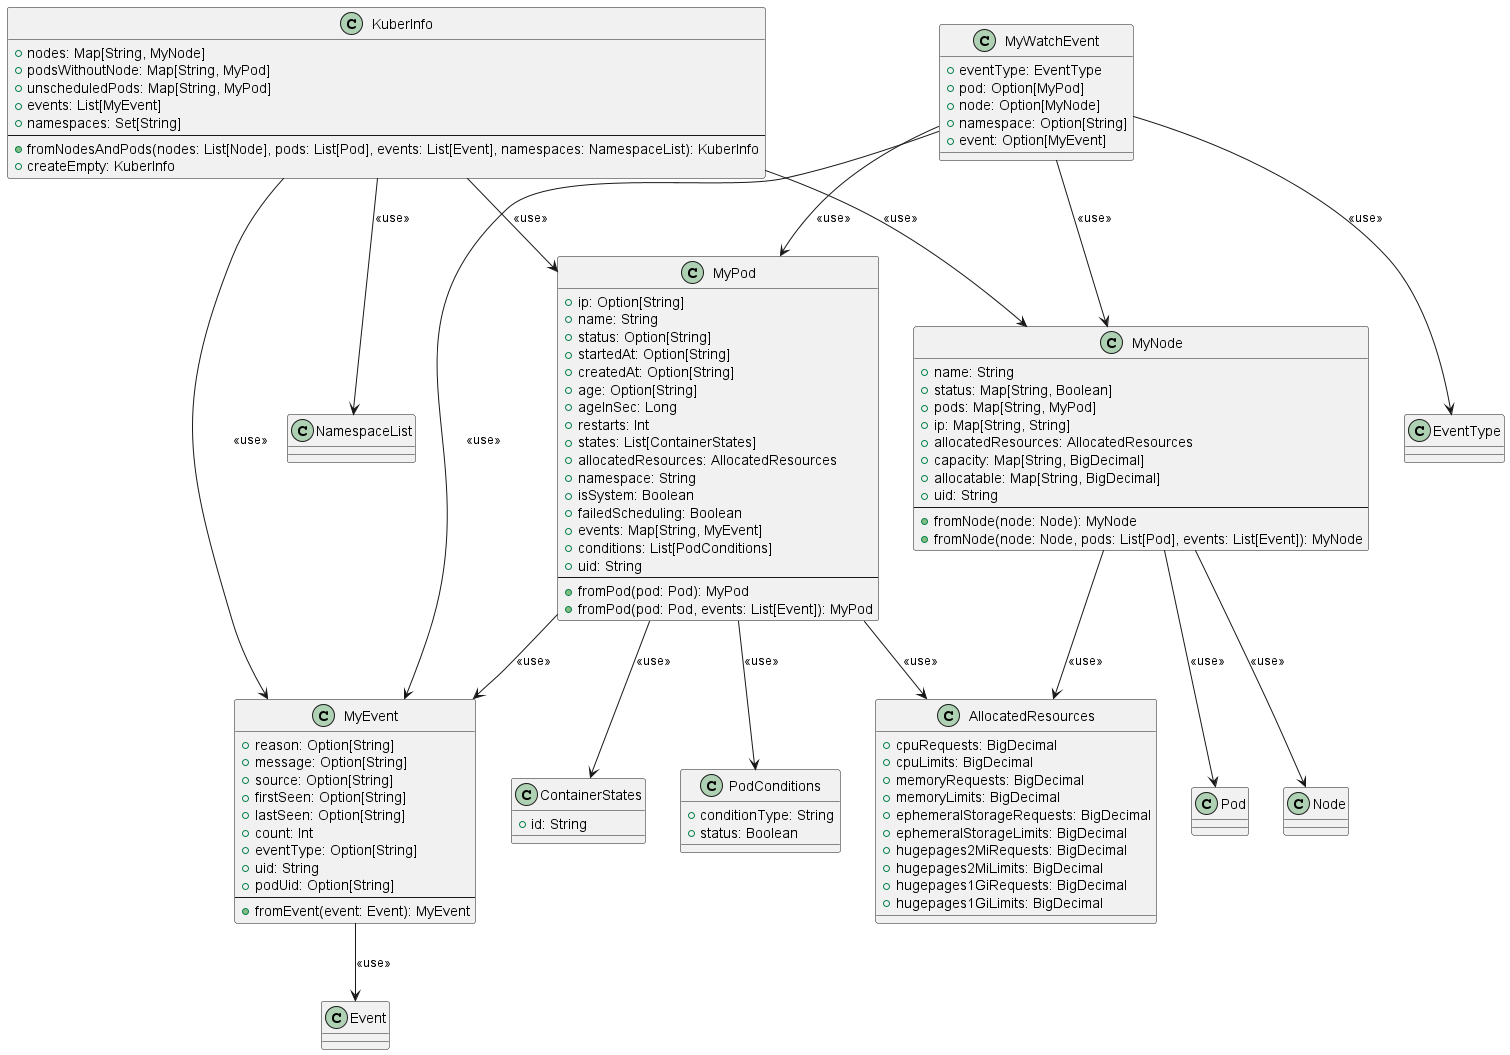
\includegraphics[scale=0.3]{img/7.png}
   \caption{Диаграмма классов модуля автомасштабирования}
   \label{fig:uml3}
  \end{figure}
  
  \subsection{Описание методов}
  
  \begin{itemize}
  \item waitUntilAllPodsVerified: Этот метод ожидает, пока все модули (поды) не
будут проверены. Он принимает следующие параметры: statefulSets (списки с
сохранением состояния) типа List[StatefulSet], deployments (развертывания) типа
List[Deployment], replicaSets (наборы реплик) типа List[ReplicaSet],
pollInterval (интервал опроса) типа FiniteDuration (по умолчанию 1 секунда),
timeout (тайм-аут) типа FiniteDuration (по умолчанию 5 минут), checkRunning
(проверять запущенные) типа Boolean (по умолчанию true).
  
  \item increaseReplicas: Этот метод увеличивает количество реплик. Он принимает
следующие параметры: resource (ресурс) типа T, где T является подтипом
ObjectResource, increment (приращение) типа Int.
  
  \item cordonNode: Этот метод блокирует узел. Он принимает следующий параметр:
nodeName (имя узла) типа String.
  
  \item getResources: Этот метод получает ресурсы.
  
  \item getAutoscaler: Этот метод получает автомасштабировщик. Он принимает
следующие параметры: namespace (пространство имен) типа String, deploymentName
(имя развертывания) типа String.
  
  \item disableAutoscaler: Этот метод отключает автомасштабировщик. Он принимает
следующие параметры: namespace (пространство имен) типа String, deploymentName
(имя развертывания) типа String.
  
  \item enableAutoscaler: Этот метод включает автомасштабировщик. Он принимает
следующий параметр: hpa (горизонтальный автомасштабировщик подов) типа
HorizontalPodAutoscaler.
  
  \item deletePod: Этот метод удаляет модуль (под). Он принимает следующие
параметры: pod (модуль) типа Pod, gracePeriod (период отсрочки) типа Int.
  
  \item processResources: Этот метод обрабатывает ресурсы. Он принимает
следующие параметры: resources (ресурсы) типа List[T], где T является подтипом
ObjectResource, nodePods (модули узла) типа List[Pod], deploymentNames (имена
развертываний) типа List[Option[String]] (по умолчанию пустой список).
  
  \item drainNodes: Этот метод освобождает узлы. Он принимает следующие
параметры: nodeNames (имена узлов) типа List[String], gracePeriod (период
отсрочки) типа Int.
  \end{itemize}
  
  \section{Создание абстрактного интерфейса для Яндекс Облака}
  
  Для обеспечения генерации конфигураций Terraform для провайдера Яндекс Облака
мы определяем абстрактный интерфейс и конкретную реализацию для этого
провайдера.
  
  \begin{minted}{scala}
  trait TerraformConfigGenerator[P] {
   def generateClusterConfig(
     servers: Seq[Server],
     masterNode: Option[Server]
   ): String
  }
  \end{minted}
  
  \subsection{Определение сервера}
  
  Тип Server теперь включает флаг для головного (master) узла.
  
  \begin{minted}{scala}
  case class Server(
   cores: Int,
   memory: Int,
   storageSize: Int,
   providerType: ProviderType,
   isMaster: Boolean = false
  )
  \end{minted}
  
  \subsection{Тип провайдера}
  
  Перечисление для типа провайдера.
  
  \begin{minted}{scala}
  enum ProviderType {
   case Yandex
  }
  \end{minted}
  
  \subsection{Реализация для Яндекс Облака}
  
  Конкретная реализация для Яндекс Облака.
  
  \begin{minted}{scala}
  class YandexConfigGenerator extends
TerraformConfigGenerator[ProviderType.Yandex.type] {
   override def generateClusterConfig(
     servers: Seq[Server],
     masterNode: Option[Server]
   ): String = {
     // Логика генерации конфигурации кластера для Яндекс Облака
   }
  }
  \end{minted}
  
  \subsection{Использование абстракции}
  
  Пример использования абстракции для генерации конфигурации кластера.
  
  \begin{minted}{scala}
  val servers = Seq(
   Server(4, 16, 100, ProviderType.Yandex, isMaster = true),
   Server(2, 8, 50, ProviderType.Yandex)
  )
  
  val configGenerator: TerraformConfigGenerator[ProviderType.Yandex.type] =
   new YandexConfigGenerator()
  
  val yandexClusterConfig = configGenerator.generateClusterConfig(
   servers,
   servers.find(_.isMaster)
  )
  \end{minted}
  
  \section{Создание системы автомасштабирования}
  
  В этом разделе описывается, как была реализована система автомасштабирования,
объединяющая генератор конфигурации Terraform (HCL) (с его абстракцией) и модуль
автомасштабирования Kubernetes.
  
  \subsection{Объединение генератора конфигурации Terraform (HCL) с модулем
автомасштабирования Kubernetes}
  
  Абстракция над генератором конфигурации Terraform (HCL) позволяет генерировать
конфигурации для облачного провайдера Яндекс Облако. Для поддержки
автомасштабирования в Kubernetes мы расширили эту абстракцию, включив в неё
возможность определения параметров для создания и управления ресурсами
Kubernetes, включая настройку горизонтального автомасштабировщика подов
(Horizontal Pod Autoscaler, HPA).
  
  \subsubsection{Интеграция с программным интерфейсом Kubernetes}
  
  Для взаимодействия с программным интерфейсом Kubernetes был разработан
отдельный модуль на Scala, который предоставляет функционал для управления
ресурсами кластера, включая создание и удаление модулей (подов), узлов и
автомасштабировщиков. Этот модуль включает в себя различные классы и методы,
такие как increaseReplicas (увеличить количество реплик), cordonNode
(заблокировать узел), getAutoscaler (получить автомасштабировщик) и другие.
  
  \subsubsection{Автомасштабирование}
  
  Система автомасштабирования была настроена для мониторинга загрузки процессора
(CPU) и памяти модулей (подов) в кластере. При достижении определённых порогов
загрузки модуль программного интерфейса Kubernetes активирует горизонтальный
автомасштабировщик подов (HPA) для автоматического увеличения или уменьшения
количества модулей (подов) в соответствии с текущими потребностями. Это
обеспечивает эффективное распределение ресурсов и оптимизацию работы приложений.
  
  \subsubsection{Генерация конфигурации Terraform}
  
  Генератор конфигурации Terraform (HCL) использует данные из модуля Kubernetes
для создания конфигураций Terraform, соответствующих текущему состоянию и
требованиям кластера Kubernetes. Например, если система автомасштабирования
решает, что необходимо больше ресурсов, генератор конфигурации Terraform (HCL)
автоматически создаёт и применяет соответствующие изменения в конфигурации
Terraform для обеспечения дополнительных ресурсов в облаке.
  
  \subsection{Пример работы системы}
  
  Предположим, что в кластере Kubernetes наблюдается высокая загрузка процессора
(CPU). Система автомасштабирования определяет необходимость увеличения
количества модулей (подов) для одного из микросервисов. Эта информация
передаётся в генератор конфигурации Terraform (HCL), который генерирует и
применяет соответствующие изменения в конфигурации Terraform для запуска
дополнительных экземпляров модулей (подов) в облачной среде.
  
  Этот процесс обеспечивает гибкое и динамическое управление ресурсами, позволяя
системе масштабироваться в соответствии с текущими потребностями, обеспечивая
при этом оптимальную производительность и стабильность работы приложений.
  
  \section{Тестирование системы автомасштабирования}
  
  Для проверки работоспособности и эффективности доработанной системы
автомасштабирования было проведено всестороннее тестирование в реальной облачной
среде Яндекс Облако. Тестирование проводилось по следующему расширенному
сценарию:
  
  \begin{enumerate}
    \item Настройка тестовой среды в Яндекс Облаке, включая создание необходимых
ресурсов и сервисов.
    \item Развертывание кластера Kubernetes с использованием обновленной
конфигурации Terraform, сгенерированной доработанным HCL генератором. Кластер
состоит из одной master ноды и трех worker нод, каждая из которых имеет 4 vCPU и
8 ГБ ОЗУ.
    \item Верификация правильности конфигурации кластера с помощью kubectl и
разработанного модуля на Scala для взаимодействия с Kubernetes API.
    \item Развертывание тестового приложения, состоящего из нескольких
микросервисов, в кластере Kubernetes. Каждый микросервис имеет свои требования к
ресурсам и политики автомасштабирования, определенные в конфигурации Terraform.
    \item Симуляция различных сценариев нагрузки на приложение, включая периоды
высокой и низкой активности пользователей. Для этого используются инструменты
нагрузочного тестирования, такие как Apache JMeter и Gatling.
    \item Мониторинг поведения системы автомасштабирования в режиме реального
времени с помощью инструментов мониторинга Kubernetes, таких как Prometheus и
Grafana. Проверяются следующие аспекты:
      \begin{itemize}
        \item Своевременное обнаружение системой изменений в нагрузке на
приложение и принятие решений о масштабировании.
        \item Корректность выполнения операций масштабирования, включая
добавление и удаление нод, а также перераспределение подов между нодами.
        \item Обеспечение желаемого уровня производительности и доступности
приложения в условиях меняющейся нагрузки.
      \end{itemize}
    \item Проверка согласованности состояния кластера Kubernetes и конфигурации
Terraform. Убедитесь, что изменения, внесенные системой автомасштабирования,
корректно отражены в обеих системах.
    \item Тестирование сценариев восстановления после сбоев, таких как отказ
ноды или сбой контейнера. Проверьте, что система автомасштабирования способна
обнаруживать и автоматически восстанавливать сервис в таких ситуациях.
    \item Оценка эффективности использования ресурсов и затрат в облаке.
Проанализируйте, насколько оптимально система автомасштабирования управляет
ресурсами и минимизирует затраты без ущерба для производительности и доступности
приложения.
   \end{enumerate}
   
   Результаты тестирования показали, что доработанная система
автомасштабирования успешно справляется с динамическим управлением ресурсами
кластера Kubernetes в соответствии с меняющимися потребностями приложения.
Улучшенный алгоритм автомасштабирования и оптимизированная модель данных
позволили системе быстрее и точнее реагировать на изменения нагрузки,
обеспечивая при этом стабильную производительность и доступность сервисов.
   
   Кроме того, тесты подтвердили согласованность состояния между кластером
Kubernetes и конфигурацией Terraform, что упрощает управление и отладку
инфраструктуры. Система также продемонстрировала устойчивость к сбоям и
способность автоматически восстанавливать сервис в случае отказа компонентов.
   
   Анализ эффективности использования ресурсов и затрат показал, что
доработанная система автомасштабирования оптимизирует потребление облачных
ресурсов, минимизируя при этом затраты без ущерба для качества обслуживания. Это
достигается за счет точного выделения ресурсов в соответствии с фактическими
потребностями приложения и своевременного освобождения неиспользуемых ресурсов.
   
   В целом, всестороннее тестирование подтвердило, что усовершенствования,
внесенные в систему автомасштабирования, значительно повысили ее эффективность,
надежность и экономичность. Доработанная система готова к развертыванию в
производственной среде и способна обеспечить оптимальное управление ресурсами и
высокую доступность приложений в условиях динамических нагрузок в облаке Яндекс.

\section{Выводы}

Созданная система автомасштабирования объединяет в себе гибкость абстракции над
HCL генератором и эффективность модуля автоскейлинга Kubernetes, обеспечивая тем
самым удобное и мощное решение для управления инфраструктурой и ресурсами в
облачных средах.

\clearpage

\chapter*{Заключение}
\addcontentsline{toc}{chapter}{Заключение}

В рамках продолжения этого учебно-исследовательского проекта была осуществлена
апробация системы автомасштабирования кластера Kubernetes на платформах РУСТЭК и
Яндекс Облако. Были детально изучены и адаптированы инструменты для
развертывания контейнеризированных сред, с акцентом на интеграцию с Terraform и
Scala. Особое внимание было уделено разработке алгебраической модели для
представления определений Terraform, включая типы данных и структуры, а также
функции для их обработки.

Разработана архитектура модуля-обертки обеспечила эффективное развертывание
типизированных определений Terraform, поддерживая генерацию HCL конфигураций и
обеспечивая взаимодействие с Kubernetes и Terraform. Реализация включала
создание парсера для плагинов Terraform, парсера документации и модуля Case
Classes Generator, а также модуля для работы с Kubernetes API.

Тестирование разработанных модулей показало их высокую эффективность и
надежность в условиях реального времени на платформах РУСТЭК и Яндекс Облако.
Однако, для достижения полной автоматизации процесса развертывания и настройки
кластера Kubernetes, требуется дополнительная разработка модуля, который будет
осуществлять изначальную развертку кластера и его настройку. Важно отметить, что
текущие модули были протестированы вручную, что подчеркивает необходимость
дальнейшей автоматизации процесса.

В целом, результаты проекта демонстрируют значительный потенциал для
автоматизации и оптимизации процессов развертывания и масштабирования приложений
в облачных средах. Для полного реализации потенциала системы и обеспечения её
надежности и удобства использования, необходимо продолжить разработку и
тестирование дополнительных модулей, особенно тех, которые отвечают за начальную
развертку и настройку кластера.


\clearpage

\phantomsection
%\addcontentsline{toc}{chapter}{\bibname}	% Добавляем список литературы в оглавление
\bibliography{chapters/biblio}						% Подключаем BibTeX-базы

%\addcontentsline{toc}{section}{Список литературы}
%\begin{thebibliography}{99}


%\bibitem{RCO1} {Ермаков А.Е.  Автоматизация онтологического инжиниринга в системах извлечения знаний из текста. М.: ООО ``ЭР СИ О'', Компьютерная лингвистика и интеллектуальные технологии: труды Международной конференци Диалог'2008, 2008.}


%\bibitem{Troel} {Троелсен Э. Язык программирования C\# 2008  и платформа .Net 3.5  М.: издательство <<Вильямс>>{}, 2010. 1344 с.}


%\bibitem{PBIRCH}{Ashwani Garg, Ashish Mangla, Neelima Gupta, Vasudha Bhatnagar PBIRCH: A scalable parallel clustering algorithm for incremental data. //Proceedings of 10th International Database Engineering and Applications Symposium IDEAS06, 2006}



%\end{thebibliography}


\endrefsection

\clearpage

%\chapter*{Приложения}
%\addcontentsline{toc}{chapter}{Приложения}
%\appendixtocon
%\renewcommand{\appendixname}{Приложение}
\appendix
\renewcommand{\appendixtocname}{Приложения}
\addappheadtotoc
%\titleformat{\chapter}[block]{\centering\normalfont\Large\bfseries}{\chaptername{} \thechapter.}{1ex}{}{}
\renewcommand{\chaptername}{Приложение}
%\renewcommand*\printchaptername{\Large\bfseries\appendixname~}
%\renewcommand{\thechapter}{Приложение \Alph{chapter}}
%\renewcommand{\thechaptertoc}{Приложение \Alph{chapter}}

%\renewcommand{\chaptermark}[1]{\markboth{\chaptername\ \thechapter.\ #1}{}}

%\begin{appendices}

\chapter{Основные правила форматирования}\label{app-format}
%\addcontentsline{toc}{chapter}{}

Текст пояснительной записки должен готовиться для печати на листах формата А4, использоваться должен шрифт с засечками (Roman; обычно --- Times Roman или Times New Roman), 12 или 14 кегль. Размеры полей:

\begin{itemize}
	\item верхнее: 20 мм.
	\item нижнее: 20 мм.
	\item левое: 10 мм.
	\item правое: 25 мм.
\end{itemize}

Нумероваться должны все страницы, начиная с первой (титульной), однако сами номера следует проставлять на страницах, начиная со страницы реферата. Номер следует проставлять внизу страницу (в центре).

Заголовки оформляются тем же шрифтом, что и основной текст (т.е., соответственно, Times Roman или Times New Roman). Для заголовков первого уровня размер шрифта может быть больше размера шрифта основного текста (обычно 14-16).

Все разделы текста: реферат, оглавление, введение, три главы основного
содержания, список литературы, заключение, приложения --- должны снабжаться
содержательным заголовком и начинаться с новой страницы; сами заголовки следует
при этом центрировать (заголовки параграфов и пунктов выравниваются по ширине).
Следует обратить внимание, что заголовки всех разделов, кроме трех основных
глав, регламентированы; заголовки трех основных глав должны быть содержательными
и отражать суть соответствующей главы. Названия типа <<Аналитическая часть>> и <<Теоретическая глава>> --- \textit{недопустимы}.

Текст пояснительной записки может содержать рисунки и таблицы. Все рисунки и
таблицы должны снабжаться номерами и подписями:

\begin{itemize}

	\item нумерация рисунков и таблиц должна быть сквозная (но раздельная, т.к. для рисунков своя, для таблиц --- своя);

	\item в случае большого количества иллюстраций/таблиц, допускается <<вложенная>> нумерация (т.е. таблицу/рисунок можно снабжать составным номером в формате 
	
	$$\langle\mbox{номер главы}\rangle.\langle\mbox{номер внутри главы}\rangle;$$
	
	\item подрисуночная подпись должна располагаться снизу по центру;
	
	\item название таблицы следует помещать над таблицей слева, без абзацного
	отступа в одну строку с ее номером через тире (ГОСТ 7.32-2001, п.6.6.1).

\end{itemize}

Здесь перечислены не все, а лишь основные требования к оформлению. Прочие
требования --- см. соответствующие ГОСТы.

Для того чтобы избежать больших отступов в списках, которые по умолчанию добавляют окружения \texttt{itemize} и \texttt{enumerate}, следует использовать 
\texttt{compactitem} (для маркированных списков) и \texttt{compactenum} (для нумерованных списков) из пакета \texttt{paralist}. 
Например:

\begin{compactitem}
	\item это;
	\item не нумерованный;
	\item список;
	\item без лишних промежутков.
\end{compactitem}

И для нумерованных списков:

\begin{compactenum}[1)]
	\item нумерованные списки;
	\item пакета \texttt{paralist};
	\item еще и удобно настраивать;
	\item (например, менять формат номера).
\end{compactenum}

\noindent или

\begin{compactenum}[a)]
	\item это другой;
	\item нумерованный;
	\item список;
	\item без лишних промежутков;
	\item и с буквенной нумерацией.
\end{compactenum}

А если хочется нумерацию сделать ангоязычной, то нужно использовать окружение \texttt{other\-language} (таким образом: \verb|\begin{otherlanguage}[numerals=latin]{russian}|)

\setkeys{russian}{numerals=latin}
%\selectlanguage{russian}
%\begin{otherlanguage}[numerals=latin]{russian}
\begin{russian}
\begin{compactenum}[a)]
	\item это другой;
	\item нумерованный;
	\item список;
	\item без лишних промежутков;
	\item и с буквенной нумерацией.
\end{compactenum}
\end{russian}
%\end{otherlanguage}

\textbf{Замечание.} По неизвестным причинам, переключения не происходит, хотя должно.

\clearpage

\chapter{Общая структура пояснительной записки}\label{app-structure}
%\addcontentsline{toc}{chapter}{}

\refsection

\begin{enumerate}
	\item Титульный лист %(в данном примере используется титульный лист от преддипломной практики)
	\item Лист с подписями (только для ВКР)
	\item Задание (в данном примере используется задание на диплом)
	\item Отчет из Интиплагиага \footnote{Обычно, допускается до 30\% заимствованного текста для работ бакалавров и до 20\% -- для работ магистров; см. соответствующие нормативные документы}
	\item Реферат (всегда на отдельной стр.)%, и эта страница \textit{НЕ} нумеруется)
	\item Оглавление. Начинается с новой страницы. %Обычно, это первая нумеруемая страница.
	\item Введение
	\begin{enumerate}
		\item Актуальность
		\item Новизна
		\item Оригинальная суть исследования
		\item Содержание ПЗ по главам (тезисно)
	\end{enumerate}
	\item Аналитическая глава. Пишется в стиле \textit{аналитического обзора}
	\item Теоретическая и инженерная глава. Описываются использованные, доработанные и разработанные модели, алгоритмы, методы, и т.п. Кроме того, тут формулируется архитектура системы.
	\item Инженерная глава. В этой главе следует отразить результаты проектирования, что, в общем случае, включает в себя следующие пункты:
	\begin{enumerate}
		\item Описание используемой методики проектирования
		\item Общая архитектура системы
		\item Архитектура подсистемы [таких подразделов может быть несколько штук, по одному на каждую подсистему или модуль, требующую детальное рассмотрение]
		\item Проектирование внешних и внутренних интерфейсов/протоколов взаимодействия
	\end{enumerate}
	\item Практическая глава. Описывается реализация, включая выбор инструментальных средств \footnote{В тех случаях, когда \begin{inparaenum}[(a)]\item этот выбор имеет существенное значение для всей работы и \item он не был, по каким-либо причинам, проделан в аналитической главе \end{inparaenum}}. Типовое содержание:
	\begin{enumerate}
		\item Состав и структура реализованного ПО 
		\item Выбор инструментальных средств
		\item Основные сценарии работы различных категорий пользователей
		\item Результаты тестирования (разработка тестовых примеров, таблицы и графики результатов прогона)
		\item Сравнение с существующими аналогами
	\end{enumerate}
	\item Заключение
	\item Список литературы 
	\item Приложения
\end{enumerate}

Кроме того, в ПЗ могут включаться и такие разделы, как словарь терминов, 
список сокращений и др. В зависимости от предпочтений автора, могут 
помещаться как в начале ПЗ (до оглавления), так и в конце (после заключения, 
но до приложений).

\paragraph{Замечания}: \mynobreakpar %\nopagebreak

\begin{enumerate}

  \item На каждый элемент из списка литературы должна быть хотя
бы одна ссылка в тексте.

  \item Список литературы должен быть оформлена согласно ГОСТ
\cite{Gost.7.1.2003,Gost.7.0.5.2008}.

  \item Минимальное количество источников для УИРов --- 15--20 (для
работ с большой аналитической и теоретической частью нормальное количество ---
25-30 и более), для дипломов --- соответственно, 30--35 и 35--60. Эти цифры
существенны, т.к. <<недобор>>, как правило, свидетельствует о не выполнении
аналитической части работы и, следовательно, недостаточном владении предметом.

  \item При подготовке РСПЗ рекомендуется вставлять уже наработанные к 
моменту подготовки РСПЗ материалы. Однако, в любом случае, каждый раздел 
должен начинаться с аннотации, заключенной в окружение \verb|\annotation|. В 
пояснительной записке к диплому аннотации не нужны. 

  \item Между заголовком главы и первым разделом рекомендуется поместить один-два абзаца связанного текста с кратким содержанием (планом) главы.

  \item Общее число и объем приложений не ограничивается. Объем ПЗ
\textbf{\textit{без}} приложений --- 25--40 стр. для УИРов, и не менее 60--100
стр. для дипломов. Объем ПЗ не может быть меньше указанных размеров. Это
означает, что студент не выполнил работу, или, как минимум, не удосужился
подготовить адекватную ПЗ. Превышать верхние пределы также не желательно, в
некоторых комиссиях это может восприниматься негативно; однако, в целом,
небольшое превышение допустимо, если проделана действительно большая работа и
получено много результатов (например, экспериментальных, или получены
нетривиальные аналитические или теоретические результаты).

  \item ГОСТ требует, чтобы нумерация страниц начиналась с 
первой, титульной, страницы. При этом на самой титульной странице номер не 
печатается. В данном случае, номера также не проставляются на листах задания, 
а также на листе с подписями (для ВКР).

\end{enumerate}

\printbibliography[heading=subbibliography]

\endrefsection


\clearpage

\chapter{Правила использования шаблона}\label{app-manual}

Настоящий шаблон все еще несколько несовершенен в плане оформления: например, неправильная нумерация приложений, и еще несколько нюансов. В последующих версиях это будет исправляться.

Ниже описана структура исходных текстов шаблона (и, соответственно, структура исходных текстов ПЗ).

Головной файл --- \texttt{thesis-template.tex}. Его задача --- <<склеить>> вместе разные части ПЗ. Каждая часть (реферат, введение, каждая содержательная глава, заключение, библиография, приложения) выделяется в отдельный файл. 

\begin{itemize}
	\item[] \texttt{thesis-macro.tex} --- содержит определения различных макрокоманд, которые часто используются в конкретной работе, например, определения окружения для теорем, некоторые часто используемые формулы, и т.п.;
	\item[] \texttt{thesis-abstract.tex} --- содержит аннотацию;
	\item[] \texttt{thesis-intro.tex} --- содержит введение;
	\item[] \texttt{thesis-chapter1.tex} --- текст первой главы;
	\item[] \texttt{thesis-chapter2.tex} --- текст второй главы;
	\item[] \texttt{thesis-chapter3.tex} --- текст третьей главы;
	\item[] \texttt{thesis-bibl.tex} --- список литературы (только подключение к
	проекту);
	\item[] \texttt{biblio.bib} --- собственно библиография (в формате BibTeX);
	\item[] \texttt{thesis-conclusion.tex} --- заключение;
	\item[] \texttt{thesis-appendix1.tex} --- первое приложение;
	\item[] \texttt{thesis-appendix2.tex} --- второе приложение;
\end{itemize}


%Одна из первых вещей, которые необходимо сделать при использовании данного шаблона --- это отредактировать аргумент команды \verb|\headertext| в начале головного файла.

Головной файл нужно менять лишь тогда, когда нужно добавить в проект новый файл, или удалить существующий (см. команду \verb|\input|). Обычно, это требуется, когда нужно добавить/удалить приложения.

Для того, чтобы \LaTeX{} при компиляции автоматически <<подхватил>> задание, его нужно сохранить в формате pdf (например, с помощью вирутального принтера), поместить в ту же папку \texttt{/title} и назвать \texttt{task.pdf}. Точно также следует поступить с титульной страницей (\texttt{title.pdf}). При оформлении ПЗ для ВКР следует дополнительно поместить в папку \texttt{/title} pdf-версию листа с подписями, назвав файл \texttt{title-dep22.pdf}. После этого, нужно раскомментировать команду \verb|
\includepdf[pages={-}, offset=0mm -0mm]{title/title-dep22.pdf}| в начале головного файла. Образцы и Word-шаблоны титульных листов для (РС)ПЗ к УИРам, НИРам, практикам и ВКР лежат в папках \texttt{/title/магистры} и \texttt{/title/бакалавры}.

В этой версии шаблона используется BibTeX, поэтому для оформления списка
литературы используются два файла: \texttt{thesis-bibl.tex} и
\texttt{biblio.bib}. Использование BibTex дает ряд преимуществ. Не нужно
заботиться о порядке сортировки, это делается автоматически; не нужно заботиться,
на какие элементы библиографии есть ссылки --- печатаются только использованные в
тексте элементы. Кроме того, многие курсовые проекты выполняются на протяжении ряда лет. С BibTex проще собирать список литературы и управлять им.

\textbf{Замечание}. В шаблоне используется пакет \texttt{hyperref}, который делает две вещи: все перекрестные ссылки <<кликабельны>>, а также выделены (красной) рамочкой. Эти рамки \textit{не выводятся на печать}. Вместо цветных рамок, возможны другие способы выделения ссылок (см. документацию пакета).


%\end{appendices}

\end{document}



